% Memoria del TFG · Diego Salas · FIB-UPC
% Compilar desde esta carpeta con:  tectonic main.tex   (o ./compilar.sh)

\documentclass[11pt,a4paper,oneside]{report}

% --- Idioma y tipografía (XeTeX, que es el motor de Tectonic) ---------------
\usepackage{fontspec}
\usepackage[catalan,english,main=spanish]{babel}
\addto\captionsspanish{%
  \renewcommand{\tablename}{Tabla}%
  \renewcommand{\listtablename}{Índice de tablas}%
  \renewcommand{\listfigurename}{Índice de figuras}%
  \renewcommand{\contentsname}{Índice}%
  \renewcommand{\bibname}{Bibliografía}}
% Fuente: Latin Modern, la que fontspec usa por defecto.

% --- Página -----------------------------------------------------------------
\usepackage[a4paper,top=2.5cm,bottom=2.5cm,left=2.5cm,right=2.5cm,headheight=14pt]{geometry}
\usepackage{setspace}
\setstretch{1.15}
\setlength{\parskip}{0.5em}
\setlength{\parindent}{0pt}

% --- Tablas, figuras y color ------------------------------------------------
\usepackage{graphicx}
\usepackage[table]{xcolor}
\usepackage{array,booktabs,longtable,tabularx,xltabular}
\usepackage{float}
\usepackage[section]{placeins}   % las tablas y figuras no saltan a otro apartado
\renewcommand{\topfraction}{0.9}
\renewcommand{\bottomfraction}{0.8}
\renewcommand{\textfraction}{0.07}
\renewcommand{\floatpagefraction}{0.75}
\usepackage[font=small,labelfont=bf,labelsep=period,skip=6pt]{caption}
\definecolor{cabeceratabla}{gray}{0.85}
% Numeración global (Tabla 1…40, Figura 1…4), como en el Google Doc
\counterwithout{table}{chapter}
\counterwithout{figure}{chapter}
\renewcommand{\arraystretch}{1.25}
% El tamaño de letra de cada tabla (\small o \footnotesize) lo fija el grupo que la rodea.
\setlength{\LTpre}{8pt}
\setlength{\LTpost}{8pt}

% --- Títulos y cabeceras ----------------------------------------------------
\usepackage{titlesec}
\titleformat{\chapter}[hang]{\huge\bfseries}{\thechapter.}{0.6em}{}
\titlespacing*{\chapter}{0pt}{0pt}{1.2em}
\setcounter{secnumdepth}{3}
\setcounter{tocdepth}{2}
\usepackage{fancyhdr}
\pagestyle{fancy}
\fancyhf{}
\fancyhead[L]{\small\nouppercase{\leftmark}}
\fancyfoot[C]{\thepage}
\renewcommand{\headrulewidth}{0.4pt}
\fancypagestyle{plain}{\fancyhf{}\fancyfoot[C]{\thepage}\renewcommand{\headrulewidth}{0pt}}

% --- Otros ------------------------------------------------------------------
\usepackage{etoolbox}
\usepackage{needspace}
\usepackage{cite}
\usepackage{tcolorbox}
\usepackage[hidelinks]{hyperref}
\usepackage{xurl}

% Marcas para lo que falta por completar (se ven en rojo en el PDF)
\newcommand{\pendiente}[1]{\textcolor{red!70!black}{\textbf{[#1]}}}
\newcommand{\figurapendiente}[1]{%
  \fcolorbox{red!60!black}{yellow!25}{\parbox[c][4cm][c]{0.8\textwidth}{\centering\pendiente{#1}}}}

% Caja para los apartados que la directora dé por cerrados (sin usar todavía)
\newtcolorbox{apartadoterminado}{colback=green!6,colframe=green!45!black,
  title={\checkmark\ Apartado terminado},fonttitle=\bfseries\small}

% --- Datos del trabajo ------------------------------------------------------
\newcommand{\titulotfg}{Selección del CRM más adecuado para el control seguro de actividades extraescolares en primaria}
\newcommand{\autortfg}{Diego Salas}

\hypersetup{pdftitle={\titulotfg},pdfauthor={\autortfg}}

\begin{document}

% ============================================================================
% Portada
% ============================================================================
\begin{titlepage}
  \centering
  
\includegraphics[width=0.75\textwidth]{imagenes/logo_upc_fib.png}\par
  \vspace{2cm}
  {\Large UNIVERSITAT POLITÈCNICA DE CATALUNYA\par}
  \vspace{0.3cm}
  {\large Facultat d'Informàtica de Barcelona (FIB)\par}
  \vspace{1.5cm}
  {\Large Trabajo Final de Grado\par}
  \vspace{1cm}
  {\LARGE\bfseries \titulotfg\par}
  \vspace{1cm}
  {\large GEP\par}
  {\large Entregable 4 - Documento final\par}
  \vfill
  \begin{tabular}{@{}>{\bfseries}l l@{}}
    Estudiante                 & Diego Salas \\
    Directora del TFG          & Carme Martín Escofet \\
    Tutora de GEP              & Giovanna Lara \\
    Titulación                 & Grado en Ingeniería Informática \\
    Especialidad               & Sistemas de Información \\
    Fecha prevista de entrega  & 12 de octubre de 2026 \\
  \end{tabular}
  \vspace{1cm}
\end{titlepage}

\pagenumbering{roman}

% ============================================================================
% Resúmenes (vacíos en la memoria original)
% ============================================================================
\chapter*{Resum}
\begin{otherlanguage}{catalan}
\pendiente{Pendent de redactar.}
\end{otherlanguage}

\chapter*{Resumen}
\pendiente{Pendiente de redactar.}

\chapter*{Summary}
\begin{otherlanguage}{english}
\pendiente{To be written.}
\end{otherlanguage}

% ============================================================================
% Índices (se generan solos, con sus números de página)
% ============================================================================
\tableofcontents
\listoftables
\listoffigures

\cleardoublepage
\pagenumbering{arabic}

% ============================================================================
% Capítulos
% ============================================================================
% Generado por trabajo_en_curso/week5/latex/convertir.py a partir del .docx de la memoria.
% A partir de ahora este fichero es la fuente: edítalo directamente.

\chapter{Contexto}\label{sec:1}

\needspace{6\baselineskip}
\section{Contextualización e introducción}\label{sec:1-1}

\needspace{6\baselineskip}
\subsection{Marco del proyecto y conceptos fundamentales}\label{sec:1-1-1}

Este Trabajo de Final de Grado se desarrolla en la especialidad de Sistemas de Información del Grado en Ingeniería Informática de la Facultad de Informática de Barcelona. El proyecto estudia la gestión de actividades extraescolares en un centro de educación primaria y evalúa la selección y adaptación de una plataforma CRM para cubrir tres procesos críticos: el control de asistencia, la trazabilidad de la custodia de los alumnos y la comunicación de incidencias.

La propuesta es aplicable a centros públicos, concertados o privados, ya que se centra en procesos comunes de organización y seguridad infantil. Las actividades pueden estar coordinadas por el propio centro, una asociación de familias o una entidad externa. En todos los casos intervienen familias, monitores, coordinación, administración y dirección, con necesidades de información y responsabilidades diferentes.

En este contexto, el CRM se entiende como una combinación de procesos, personas y tecnología para gestionar relaciones e interacciones de forma coherente~\cite{ref01}. El alumno es el sujeto protegido, mientras que las familias y las personas autorizadas son los contactos asociados a su ficha. Los conceptos principales del sistema son los siguientes:

\begin{itemize}
  \item \textbf{Asistencia:} registro del estado del alumno en cada sesión, incluyendo presencia, ausencia, retraso o justificación, junto con la fecha, hora y usuario que realiza el cambio.
  \item \textbf{Custodia y entrega:} registro de la responsabilidad del menor durante la actividad y de su entrega final a una persona autorizada.
  \item \textbf{Incidencia:} hecho relevante ocurrido durante una actividad, clasificado por tipo y gravedad, con actuaciones realizadas y comunicación a los destinatarios correspondientes.
  \item \textbf{Trazabilidad:} capacidad de reconstruir el historial de asistencia, custodia, incidencias y cambios realizados sobre cada alumno.
\end{itemize}

Dado que el sistema tratará datos personales de menores y de sus representantes, deberá respetar los principios de finalidad, minimización, seguridad y deber de información~\cite{ref02}. La privacidad y el control de acceso se consideran, por tanto, requisitos del sistema desde su diseño.

\needspace{6\baselineskip}
\subsection{Problema y actores implicados}\label{sec:1-1-2}

Como escenario de referencia, se plantea una gestión fragmentada: las inscripciones se mantienen en hojas de cálculo, los monitores utilizan listas independientes para pasar asistencia, las autorizaciones de recogida se comunican por correo o mensajería y las incidencias se registran o notifican mediante canales no centralizados. Este escenario deberá validarse posteriormente con el centro colaborador.

Esta fragmentación puede provocar listas desactualizadas, dificultades para confirmar si un alumno asistió o fue recogido por una persona autorizada, pérdida de información sobre incidencias y un esfuerzo manual elevado para preparar informes. Además, el uso de canales informales dificulta controlar permisos, conservación de datos y auditoría. Ahora se expondrá la tabla de actores.

\begin{table}[H]
\centering\small
\begin{tabularx}{\textwidth}{>{\hsize=0.865\hsize\raggedright\arraybackslash}X>{\hsize=0.806\hsize\raggedright\arraybackslash}X>{\hsize=1.228\hsize\raggedright\arraybackslash}X>{\hsize=1.154\hsize\raggedright\arraybackslash}X}
\toprule
\rowcolor{cabeceratabla} \textbf{Actor} & \textbf{Relación con el sistema} & \textbf{Necesidad principal} & \textbf{Acceso previsto} \\
\midrule
Dirección & Responsable organizativo & Supervisar cumplimiento, riesgos e incidencias graves & Indicadores, auditoría y escalados \\
Coordinación & Gestión diaria & Mantener grupos, sesiones, autorizaciones y seguimiento & Vista operativa completa dentro de su ámbito \\
Monitorado & Usuario de primera línea & Pasar lista, registrar entregas e incidencias & Solo actividades y alumnos asignados \\
Administración & Soporte de datos & Altas, bajas, contactos y documentación & Datos administrativos; sin detalle innecesario de incidencias \\
Familias y tutores & Origen y destinatario de información & Actualizar contactos, autorizaciones y recibir comunicaciones & Información de sus menores y acuses \\
Alumnado & Sujeto protegido y beneficiario & Participar con seguridad y recibir atención coherente & Sin acceso directo en el alcance inicial \\
Delegado de protección de datos & Control y asesoramiento & Revisar legitimación, contratos, riesgos y derechos & Evidencias y configuración, según necesidad \\
Proveedor o administrador TI & Operación técnica & Mantener disponibilidad, copias y seguridad & Acceso técnico restringido y registrado \\
Estudiante (Diego Salas) & Responsable de ejecución del TFG & Analizar, configurar, probar y documentar la propuesta & Administración del entorno de pruebas y repositorio; sin datos reales \\
Tutora de GEP & Seguimiento académico de la gestión & Revisar alcance, planificación y evidencias de gestión & Documentación y evidencias del proyecto; sin acceso operativo a datos \\
\bottomrule
\end{tabularx}
\caption{Actores implicados}\label{tab:1}
\end{table}

\needspace{6\baselineskip}
\section{Justificación de la solución}\label{sec:1-2}

\needspace{6\baselineskip}
\subsection{Justificación del TFG y antecedentes}\label{sec:1-2-1}

El problema no parte de una necesidad tecnológica abstracta. En programas con responsabilidad sobre menores, la asistencia y la entrega requieren registrar la entrada y la salida, identificar a las personas autorizadas y dejar constancia de las excepciones. Las pautas de seguridad para programas juveniles recomiendan documentar la transición de custodia, conservar la hora de llegada y salida y registrar la identidad de la persona que recoge al menor~\cite{ref31}.

También existen soluciones especializadas que cubren partes de este flujo. BatOnRoute incluye control de asistencia en actividades extraescolares y registra quién recoge al alumno, cuándo y con qué autorización~\cite{ref32}; Qualla gestiona cambios de recogida, autorizaciones y avisos a las familias~\cite{ref33}. Estos antecedentes confirman que la necesidad es real, pero no sustituyen el objetivo del TFG: estudiar de forma reproducible si un CRM configurable puede integrar asistencia, custodia e incidencias en un mismo modelo de información, con control de acceso y posibilidad de adaptación para un centro de primaria.

\needspace{6\baselineskip}
\subsection{Solución propuesta}\label{sec:1-2-2}

La solución propuesta centralizará la información en una ficha relacional del alumno. Las inscripciones generarán las listas de cada sesión; el monitor registrará la asistencia desde una interfaz web; la entrega quedará vinculada a una persona autorizada; y las incidencias seguirán un flujo con prioridad, responsable y registro de comunicación. Cada perfil accederá únicamente a los datos necesarios: los monitores gestionarán sus grupos, coordinación supervisará las actividades, administración mantendrá los datos de inscripción y dirección podrá consultar indicadores e incidencias escaladas.

La propuesta pretende mejorar la seguridad operativa y la coordinación entre los actores implicados sin sustituir la decisión humana ante una recogida excepcional. El RGPD exige aplicar medidas adecuadas al riesgo y protección de datos desde el diseño~\cite{ref03}. Por ello, el TFG analizará los procesos actuales, comparará alternativas CRM y validará una adaptación que aporte trazabilidad, control de acceso y un canal ordenado para las incidencias.

\needspace{6\baselineskip}
\subsection{Adaptar una plataforma}\label{sec:1-2-3}

Se consideran tres estrategias:

\begin{itemize}
  \item La primera es continuar con herramientas ofimáticas e introducir formularios y plantillas. Tiene un coste inicial bajo, pero mantiene la fragmentación y exige construir manualmente permisos, historial y alertas.
  \item La segunda es desarrollar una aplicación completa a medida. Ofrece control funcional, aunque consume gran parte del TFG en autenticación, administración, interfaces básicas y mantenimiento.
  \item La tercera es adaptar una plataforma con gestión de contactos, roles, flujos, API y capacidad de extensión.
\end{itemize}

La tercera estrategia es la más proporcionada. Permite dedicar el esfuerzo de ingeniería a modelar la custodia y las incidencias, que son los elementos diferenciales, y reutiliza capacidades maduras para usuarios, relaciones, notificaciones y administración. La decisión no elimina el desarrollo: exige diseñar entidades, reglas, permisos, vistas y pruebas específicas. Además, reduce el riesgo de construir un prototipo aislado que no pueda evolucionar.

Las plataformas escolares verticales se analizarán como referencia funcional, pero no serán la base prioritaria si su modelo cerrado impide estudiar y adaptar el sistema. El entregable técnico debe mostrar cómo una plataforma configurable puede transformarse para un proceso distinto del comercial y evaluar sus límites con criterios reproducibles.

\needspace{6\baselineskip}
\subsection{Alternativas preseleccionadas}\label{sec:1-2-4}

Se preseleccionan tres plataformas con enfoques diferentes. SuiteCRM 8 es un CRM de código abierto que puede instalarse en infraestructura propia y ofrece API, herramientas para crear módulos, relaciones, campos y vistas~\cite{ref05,ref06,ref07}. Odoo combina CRM con un entorno modular amplio; su documentación distingue contactos, derechos de acceso y reglas de registro, aunque su módulo estándar de asistencia está orientado a empleados y requiere adaptación para alumnado~\cite{ref10}. Salesforce Education Cloud aporta un modelo educativo amplio y relaciones entre estudiantes y tutores, pero opera como servicio propietario y su coste y dependencia del proveedor deben valorarse para un centro pequeño~\cite{ref11}.

No se incluye una plataforma solo por popularidad. Cada candidata debe permitir representar la relación alumno-familia, restringir el acceso por actividad y conservar evidencia de asistencia, custodia e incidencias. Los criterios y pesos de la Tabla~\ref{tab:2} se fijan antes de puntuar para reducir el sesgo hacia una herramienta concreta.

\begin{table}[H]
\centering\small
\begin{tabularx}{\textwidth}{>{\hsize=0.714\hsize\raggedright\arraybackslash}X>{\hsize=0.222\hsize\raggedright\arraybackslash}X>{\hsize=2.063\hsize\raggedright\arraybackslash}X}
\toprule
\rowcolor{cabeceratabla} \textbf{Criterio} & \textbf{Peso} & \textbf{Forma de evaluación} \\
\midrule
Adecuación funcional & 25 \% & Cobertura nativa o configurable de personas, relaciones, sesiones, estados y comunicaciones \\
Privacidad y seguridad & 20 \% & Roles, permisos a nivel de registro, auditoría, autenticación e implantación de medidas RGPD \\
Extensibilidad & 20 \% & Creación de módulos, reglas, API y posibilidad de mantener extensiones sin modificar el núcleo \\
Control de despliegue y datos & 15 \% & Opciones de alojamiento, exportación, copias, portabilidad y dependencia del proveedor \\
Coste y licencia & 10 \% & Licencias, infraestructura, complementos y sostenibilidad para un centro de primaria \\
Usabilidad y aprendizaje & 10 \% & Adecuación móvil, consistencia de interfaz, documentación y esfuerzo de formación \\
\bottomrule
\end{tabularx}
\caption{Criterios de selección}\label{tab:2}
\end{table}

\needspace{6\baselineskip}
\subsection{Método de evaluación}\label{sec:1-2-5}

Cada alternativa recibe una puntuación de 1 a 5 por criterio: 1 significa que no cubre la necesidad o exige una solución externa sustancial; 3 indica cobertura parcial con configuración o desarrollo asumible; y 5 representa cobertura sólida, verificable y sostenible. La puntuación total se calcula mediante la suma de cada nota multiplicada por su peso. Durante el TFG, las notas se confirmarán con una prueba de concepto equivalente para cada candidata: creación de un alumno y dos autorizados, restricción de un monitor a su grupo, registro de asistencia, alta de una incidencia y exportación del historial.

La comparación inicial se apoya en documentación oficial. SuiteCRM permite crear módulos y relaciones con Module Builder y Studio~\cite{ref07}, definir roles y grupos de seguridad~\cite{ref08} y automatizar acciones mediante workflows~\cite{ref09}. Su licencia AGPLv3 permite estudiar y modificar el código, aunque obliga a revisar las condiciones de distribución de las adaptaciones~\cite{ref06}. Estas capacidades encajan con un prototipo académico que necesita entidades nuevas y control sobre el alojamiento.

\needspace{6\baselineskip}
\subsection{Evaluación comparativa}\label{sec:1-2-6}

La Tabla~\ref{tab:3} recoge la evaluación preliminar. Las puntuaciones deberán actualizarse si la prueba de concepto contradice alguna capacidad documentada. Esta trazabilidad evita convertir la matriz en una justificación retrospectiva.

\begin{table}[H]
\centering\footnotesize
\begin{tabularx}{\textwidth}{>{\hsize=2.264\hsize\raggedright\arraybackslash}X>{\hsize=0.720\hsize\raggedright\arraybackslash}X>{\hsize=0.649\hsize\raggedright\arraybackslash}X>{\hsize=0.567\hsize\raggedright\arraybackslash}X>{\hsize=0.799\hsize\raggedright\arraybackslash}X}
\toprule
\rowcolor{cabeceratabla} \textbf{Criterio} & \textbf{Peso} & \textbf{SuiteCRM 8} & \textbf{Odoo CRM} & \textbf{Salesforce Education Cloud} \\
\midrule
Adecuación funcional & 25 \% & 3 & 3 & 4 \\
Privacidad y seguridad & 20 \% & 4 & 4 & 5 \\
Extensibilidad & 20 \% & 5 & 5 & 5 \\
Control de despliegue y datos & 15 \% & 5 & 4 & 2 \\
Coste y licencia & 10 \% & 5 & 3 & 1 \\
Usabilidad y aprendizaje & 10 \% & 3 & 4 & 4 \\
Resultado ponderado & 100 \% & 4,10 & 3,85 & 3,80 \\
\bottomrule
\end{tabularx}
\caption{Matriz ponderada de alternativas}\label{tab:3}
\end{table}

Con la información documental disponible, SuiteCRM obtiene 4,10 sobre 5 y se adopta como candidata de trabajo provisional. Su principal desventaja es la falta de objetos escolares nativos, lo que aumenta el trabajo de análisis y diseño. Esta carencia es asumible porque el objetivo del TFG incluye adaptar un CRM. No obstante, la decisión definitiva quedará condicionada a completar las pruebas de concepto equivalentes y a validar el proceso con el centro colaborador. Odoo y Salesforce se mantendrán como alternativas hasta cerrar esa validación: Odoo ofrece un marco técnico atractivo, mientras que Salesforce aporta una mayor cobertura educativa, pero sus licencias, alojamiento gestionado y dependencia del proveedor reducen su adecuación inicial a un centro pequeño.

\needspace{6\baselineskip}
\subsection{Opción tecnológica provisional}\label{sec:1-2-7}

Se trabajará inicialmente con SuiteCRM 8 en un entorno de desarrollo aislado y con un paquete de extensión denominado Gestión de Extraescolares. La decisión de mantener esta plataforma se registrará al finalizar las pruebas de concepto; si una alternativa supera los criterios críticos, se revisará la línea base antes de desarrollar los módulos. El modelo reutilizará usuarios, contactos, actividades, notificaciones y API cuando aporten valor, pero no representará a los menores como oportunidades comerciales. Se crearán módulos específicos para Alumnos, Personas autorizadas, Actividades, Grupos, Sesiones, Asistencias, Eventos de custodia e Incidencias.

Las relaciones centrales serán: un alumno puede tener varias personas autorizadas; una actividad contiene grupos y sesiones; una inscripción vincula alumno y grupo durante un periodo; cada sesión genera registros de asistencia; y cada salida genera un evento de custodia asociado al alumno, la sesión, la persona que entrega y la persona autorizada que recoge. Una incidencia podrá relacionarse con alumno, sesión y actividad, pero su visibilidad dependerá de la gravedad y el rol.

Los workflows automatizarán avisos, escalados y tareas, sin sustituir decisiones sensibles. Por ejemplo, una ausencia no generará automáticamente una acusación o alarma; creará una tarea de verificación según el protocolo acordado. La entrega a una persona no autorizada quedará bloqueada y exigirá intervención de coordinación. Las comunicaciones registrarán destinatario, canal, fecha, estado y acuse cuando proceda, evitando almacenar conversaciones privadas completas.

\needspace{6\baselineskip}
\subsection{Arquitectura y protección desde el diseño}\label{sec:1-2-8}

La aplicación se alojará sobre HTTPS con base de datos separada, copias cifradas y perfiles de mínimo privilegio. El repositorio de código solo contendrá configuración y extensiones, nunca datos reales. Para desarrollo y pruebas se usarán datos sintéticos. La minimización afectará también a la custodia: el sistema guardará la referencia de la persona autorizada y el método de comprobación, pero no una copia completa del documento de identidad salvo que exista una base jurídica y una necesidad aprobada. Esta decisión aplica los principios de los artículos 5, 25 y 32 del RGPD~\cite{ref03}.

\needspace{6\baselineskip}
\section{Alcance del proyecto}\label{sec:1-3}

\needspace{6\baselineskip}
\subsection{Objetivo general}\label{sec:1-3-1}

El objetivo general es analizar el sistema de información de las actividades extraescolares de un centro de primaria, seleccionar la plataforma CRM más adecuada y construir una adaptación que permita controlar asistencia, mantener la trazabilidad de la custodia y gestionar incidencias con seguridad, privacidad y evidencia verificable.

\needspace{6\baselineskip}
\subsection{Subobjetivos y entregables}\label{sec:1-3-2}

\begin{itemize}
  \item Validar el proceso de referencia con los interesados e identificar actores, reglas, excepciones y requisitos priorizados.
  \item Comparar alternativas mediante pruebas de concepto equivalentes y justificar la selección mediante una matriz ponderada reproducible.
  \item Diseñar e implementar el producto mínimo viable: modelo de datos, permisos, asistencia, custodia, incidencias y notificaciones.
  \item Probar la solución, documentar sus resultados y entregar configuración reproducible, datos sintéticos, manual de uso y guía técnica.
\end{itemize}

Los entregables serán el documento de análisis y requisitos, el informe de selección, el modelo de datos y permisos, el paquete de extensión para SuiteCRM y el plan con resultados de prueba. La matriz de trazabilidad relacionará cada objetivo con requisito, implementación, caso de prueba y evidencia.

\needspace{6\baselineskip}
\subsection{Límites del alcance}\label{sec:1-3-3}

Quedan fuera la gestión académica, calificaciones, facturación, contabilidad, nóminas, planificación de aulas y contratación de monitores. La solución será web adaptable, no una aplicación móvil nativa. También se excluyen la biometría y el reconocimiento facial por su impacto y falta de necesidad para el objetivo.

La primera versión probará las notificaciones en un entorno controlado y no enviará comunicaciones reales por SMS o servicios comerciales. Cualquier integración con correo o plataforma del centro requerirá una revisión contractual y de protección de datos. El sistema aplicará autorizaciones vigentes, pero el personal responsable conservará la decisión final ante una recogida excepcional.

La validación se realizará con datos sintéticos y un centro de referencia. Demostrará la viabilidad del caso definido, no una implantación general. Una puesta en producción requerirá análisis de riesgos, acuerdo con el responsable del tratamiento, formación y validación jurídica.

\needspace{6\baselineskip}
\subsection{Requisitos y riesgos}\label{sec:1-3-4}

Los requisitos del producto mínimo viable se separan en funcionales y no funcionales. Los atributos de calidad se basan en ISO/IEC 25010:2023~\cite{ref12}. La prioridad M identifica los requisitos obligatorios; S, los importantes; y C, las mejoras deseables.

Los requisitos funcionales describen las capacidades que debe ofrecer la adaptación para gestionar información, asistencia, custodia, incidencias y permisos.

\begin{table}[H]
\centering\small
\begin{tabularx}{\textwidth}{>{\hsize=0.275\hsize\raggedright\arraybackslash}X>{\hsize=1.591\hsize\raggedright\arraybackslash}X>{\hsize=0.436\hsize\raggedright\arraybackslash}X>{\hsize=1.698\hsize\raggedright\arraybackslash}X}
\toprule
\rowcolor{cabeceratabla} \textbf{ID} & \textbf{Requisito resumido} & \textbf{Prior.} & \textbf{Comprobación} \\
\midrule
RF01 & Gestionar alumnos, contactos, autorizaciones vigentes e inscripciones. & M & No se guarda una ficha incompleta; una autorización vencida o revocada no es válida. \\
RF02 & Gestionar actividades, grupos y sesiones; generar la lista de sesión desde inscripciones activas. & M & La lista excluye alumnos de otra actividad o con inscripción cancelada; inicio anterior a fin. \\
RF03 & Registrar asistencia y cambios con estado, hora, autor y motivo. & M & Cada alumno queda en un estado controlado; no hay dos registros para la misma sesión. \\
RF04 & Registrar custodia y entrega; bloquear o escalar una salida a una persona no autorizada. & M & El evento conserva sesión, responsable y receptor; solo se confirma una entrega autorizada. \\
RF05 & Tramitar incidencias por tipo, prioridad, responsable, actuación y estado. & M & No se cierra una incidencia sin responsable y actuación registrada. \\
RF06 & Registrar comunicaciones de incidencias con destinatario, canal, envío y acuse cuando exista. & M & Cada aviso queda vinculado a la incidencia; no se envía a un destinatario no autorizado. \\
RF07 & Aplicar permisos por actividad y rol y consultar o exportar historial autorizado. & M & Un monitor no accede a grupos ajenos; coordinación reconstruye una sesión con auditoría. \\
RF08 & Importar CSV validado y exportar únicamente información autorizada. & S & Los errores se informan y ninguna fila se aplica parcialmente sin confirmación. \\
RF09 & Generar indicadores agregados y habilitar un portal familiar limitado. & C & Los indicadores no exponen datos innecesarios; la familia solo consulta información de sus menores. \\
\bottomrule
\end{tabularx}
\caption{Requisitos funcionales}\label{tab:4}
\end{table}

Los requisitos no funcionales establecen las condiciones de seguridad, rendimiento, recuperación, mantenibilidad, usabilidad y accesibilidad que deberá cumplir el prototipo.

\begin{table}[H]
\centering\small
\begin{tabularx}{\textwidth}{>{\hsize=0.334\hsize\raggedright\arraybackslash}X>{\hsize=2.006\hsize\raggedright\arraybackslash}X>{\hsize=0.436\hsize\raggedright\arraybackslash}X>{\hsize=1.224\hsize\raggedright\arraybackslash}X}
\toprule
\rowcolor{cabeceratabla} \textbf{ID} & \textbf{Requisito resumido} & \textbf{Prior.} & \textbf{Comprobación} \\
\midrule
RNF01 & Seguridad y privacidad: HTTPS, acceso individual, mínimo privilegio, auditoría y datos sintéticos. & M & Pruebas de acceso indebido y revisión de exportaciones~\cite{ref02,ref03,ref04}. \\
RNF02 & Rendimiento, recuperación y mantenibilidad: \textless{}2 s en el 95 \% de operaciones; copias y extensiones versionadas. & M & Prueba con 10.000 alumnos, restauración y guía de instalación. \\
RNF03 & Usabilidad y accesibilidad: asistencia y entrega en tres acciones; WCAG 2.2 AA cuando aplique. & S & Prueba de tareas y SUS $\geq$ 68. \\
\bottomrule
\end{tabularx}
\caption{Requisitos no funcionales}\label{tab:5}
\end{table}

\begin{table}[H]
\centering\small
\begin{tabularx}{\textwidth}{>{\hsize=0.974\hsize\raggedright\arraybackslash}X>{\hsize=0.215\hsize\raggedright\arraybackslash}X>{\hsize=1.811\hsize\raggedright\arraybackslash}X}
\toprule
\rowcolor{cabeceratabla} \textbf{Riesgo} & \textbf{P/I} & \textbf{Respuesta} \\
\midrule
Requisitos sin validar & A/A & Entrevistas, prototipos y registro de supuestos; revisar reglas sin responsable. \\
Exposición de datos de menores & M/MA & Datos sintéticos, permisos mínimos y pruebas negativas de acceso. \\
Complejidad o cambios en SuiteCRM & M/A & Prueba técnica temprana y paquete desacoplado del núcleo. \\
Sobrealcance o baja adopción & A/M & MoSCoW, producto mínimo, pruebas de tareas y formación breve. \\
Fallo de notificaciones o datos & M/MA & Reintentos, canal alternativo, copias cifradas y restauración ensayada. \\
\bottomrule
\end{tabularx}
\caption{Riesgos prioritarios y respuesta}\label{tab:6}
\end{table}

El riesgo principal es partir de un escenario sin centro identificado. Cada regla se marcará como validada, pendiente o descartada. Si el centro impone un procedimiento incompatible, se revisarán la matriz de selección y la línea base del alcance.

\needspace{6\baselineskip}
\section{Metodología de trabajo y rigor}\label{sec:1-4}

\needspace{6\baselineskip}
\subsection{Enfoque metodológico}\label{sec:1-4-1}

El proyecto seguirá un ciclo de vida iterativo e incremental, apoyado por Kanban y revisiones quincenales. Se toman de Scrum la existencia de un backlog ordenado, objetivos de iteración, revisión del incremento y retrospectiva~\cite{ref13}, pero no se afirma que se aplique Scrum de forma completa. El trabajo lo realiza una sola persona y no existen un Scrum Team ni todos sus roles. Kanban permitirá limitar el trabajo en curso y visualizar tareas pendientes, activas, en revisión y terminadas, de acuerdo con el material de gestión ágil de GEP.

El alcance se controlará mediante una línea base de objetivos, requisitos y exclusiones. Una petición nueva se registrará, estimará y clasificará antes de incorporarse. Si afecta a una funcionalidad obligatoria, se revisarán tiempo y prioridad con la directora del TFG. Este procedimiento sigue la recomendación de ejecutar lo previsto, documentar cambios y justificar medidas correctoras.

\begin{table}[H]
\centering\small
\begin{tabularx}{\textwidth}{>{\hsize=0.462\hsize\raggedright\arraybackslash}X>{\hsize=1.268\hsize\raggedright\arraybackslash}X>{\hsize=1.271\hsize\raggedright\arraybackslash}X}
\toprule
\rowcolor{cabeceratabla} \textbf{Iteración} & \textbf{Trabajo principal} & \textbf{Resultado verificable} \\
\midrule
0 Contexto & Entrevistas, proceso, actores y protección de datos & Mapa validado, supuestos y registro inicial de riesgos \\
1 Requisitos & Casos, reglas, prioridades y criterios de aceptación & Backlog y matriz de trazabilidad aprobados \\
2 Selección & Pruebas de concepto y matriz ponderada & Informe reproducible y decisión registrada \\
3 Modelo & Entidades, relaciones, roles y datos sintéticos & Paquete instalable y pruebas de permisos \\
4 Núcleo & Asistencia, custodia, incidencias y workflows & Incremento demostrable con pruebas funcionales \\
5 Validación & Seguridad, rendimiento, usabilidad y recuperación & Informe de resultados, defectos y correcciones \\
6 Cierre & Documentación, despliegue y memoria & Entrega reproducible y trazabilidad completa \\
\bottomrule
\end{tabularx}
\caption{Iteraciones, resultados y evidencias}\label{tab:7}
\end{table}

\needspace{6\baselineskip}
\subsection{Seguimiento y herramientas}\label{sec:1-4-2}

El backlog y el tablero Kanban se gestionarán con GitHub Projects o una herramienta equivalente. El código y la documentación técnica se mantendrán en un repositorio privado Git, con ramas breves y revisiones antes de integrar. Las actas de reunión registrarán decisiones, cambios y tareas. Los documentos académicos usarán un gestor bibliográfico para mantener el estilo IEEE y evitar referencias sin correspondencia en el texto.

El rigor se apoyará en una matriz que relacione cada objetivo con requisitos, tareas, casos de prueba y evidencias. Un elemento solo pasará a terminado cuando cumpla su criterio de aceptación, incluya pruebas, documentación mínima y no introduzca defectos críticos. Al final de cada iteración se medirán requisitos obligatorios completados, pruebas superadas, defectos abiertos, desviación de esfuerzo y riesgos activos.

\needspace{6\baselineskip}
\subsection{Validación}\label{sec:1-4-3}

La validación combinará: pruebas unitarias para reglas; pruebas de integración para relaciones y workflows; pruebas de autorización con perfiles incompatibles; pruebas de rendimiento con datos sintéticos; restauración de una copia; y pruebas de tareas con coordinación y monitores. Las incidencias se clasificarán por severidad. La aceptación del producto mínimo exigirá que todos los requisitos M tengan evidencia, que no existan accesos indebidos conocidos y que los defectos críticos estén cerrados.

Las revisiones con la directora del TFG confirmarán alcance, decisión tecnológica e incrementos. La tutora de GEP validará la coherencia de la gestión del proyecto. Si no se dispone de usuarios reales, la evaluación de usabilidad se declarará exploratoria y se evitarán conclusiones generalizables. Esta separación entre evidencia, interpretación y limitaciones permitirá valorar el resultado con criterios transparentes.


% Generado por trabajo_en_curso/week5/latex/convertir.py a partir del .docx de la memoria.
% A partir de ahora este fichero es la fuente: edítalo directamente.

\chapter{Planificación}\label{sec:2}

\needspace{6\baselineskip}
\section{Datos globales del proyecto}\label{sec:2-1}

El inicio se sitúa el 19 de octubre de 2026, tras finalizar la fase GEP. Esta decisión evita solapar entregables académicos y permite dedicar el periodo posterior a la construcción, validación y redacción. La fecha límite operativa es el 10 de enero de 2027; por tanto, la validación funcional se completa antes de la última semana.

\begin{table}[H]
\centering\small
\begin{tabularx}{\textwidth}{>{\hsize=0.957\hsize\raggedright\arraybackslash}X>{\hsize=1.043\hsize\raggedright\arraybackslash}X}
\toprule
\rowcolor{cabeceratabla} \textbf{Parámetro} & \textbf{Valor} \\
\midrule
Inicio planificado & 19/10/2026 \\
Finalización y defensa interna & 10/01/2027 \\
Duración calendario & 12 semanas \\
Carga de trabajo base & 405 horas \\
Reserva de contingencia & 45 horas (11,1 \% de la base) \\
Dedicación prevista & 37,5 horas semanales de media \\
Método de ejecución & 4 sprints de 3 semanas \\
Hitos & Requisitos, CRM seleccionado, prototipo, validación y cierre \\
\bottomrule
\end{tabularx}
\caption{Parámetros de planificación}\label{tab:8}
\end{table}

\needspace{6\baselineskip}
\subsection{Criterios de estimación}\label{sec:2-1-1}

Las estimaciones se expresan en horas y se han descompuesto en tareas de tamaño manejable. Las tareas de construcción se han dimensionado entre 14 y 45 horas, manteniéndose por debajo del umbral de 50 horas. La suma de tareas ordinarias es 405 horas. Las 45 horas de contingencia se mantienen diferenciadas del trabajo base, pero forman parte de la capacidad total planificada de 450 horas. Esto sumado a las 90 horas de GEP dan un total de 540 horas de TFG.

\needspace{6\baselineskip}
\subsection{Seguimiento}\label{sec:2-1-2}

Al cierre de cada semana se actualizarán horas reales, tareas terminadas, impedimentos y fecha estimada de los hitos. Al final de cada sprint se realizará una revisión del incremento: primero requisitos y selección, después configuración, posteriormente adaptación de módulos y finalmente pruebas. Si una tarea crítica se retrasa más de cuatro horas, se aplicará el plan alternativo correspondiente.

\needspace{6\baselineskip}
\subsection{Calendario y dedicación}\label{sec:2-1-3}

El calendario considera la disponibilidad del estudiante, los festivos previsibles y la necesidad de reservar las validaciones con terceros fuera del periodo navideño. La carga base equivale a 33,75 horas semanales y la contingencia reserva 3,75 horas semanales de capacidad no asignada. La dedicación total prevista es, por tanto, de 37,5 horas semanales. Esta distribución permite que los hitos tengan evidencia disponible antes de la revisión de cada sprint y evita concentrar la memoria técnica al final del proyecto.

\needspace{6\baselineskip}
\section{Especificación y descripción de tareas}\label{sec:2-2}

La EDT se organiza en siete paquetes: gestión, análisis, selección, diseño y configuración, adaptación, validación y cierre. Las precedencias se indican con la notación Tn \textless{} Tm, que significa que la tarea Tn debe finalizar antes de iniciar Tm. Los recursos son el estudiante, la dirección y tutoría, usuarios de validación y un entorno de pruebas con SuiteCRM.

\begin{table}[H]
\centering\footnotesize
\begin{tabularx}{\textwidth}{>{\hsize=0.500\hsize\raggedright\arraybackslash}X>{\hsize=2.223\hsize\raggedright\arraybackslash}X>{\hsize=0.260\hsize\raggedright\arraybackslash}X>{\hsize=0.874\hsize\raggedright\arraybackslash}X>{\hsize=1.144\hsize\raggedright\arraybackslash}X}
\toprule
\rowcolor{cabeceratabla} \textbf{Código} & \textbf{Tarea} & \textbf{h} & \textbf{Precedencia} & \textbf{Recursos} \\
\midrule
T1 & Planificación detallada, seguimiento semanal y control de cambios & 25 & — & Estudiante, dirección \\
T2 & Definir actores, necesidades y casos de uso del centro & 18 & — & Estudiante, usuarios \\
T3 & Modelar proceso actual, requisitos y protección de datos & 28 & T2 & Estudiante, usuarios \\
T4 & Establecer criterios, preselección y pruebas de concepto CRM & 16 & T3 & Estudiante, fuentes técnicas \\
T5 & Comparar candidatos y justificar la selección de SuiteCRM & 16 & T4 & Estudiante, entorno de prueba \\
T6 & Diseñar modelo de datos, roles, permisos y trazabilidad & 30 & T3 \textless{} T6; T5 \textless{} T6 & Estudiante, dirección \\
T7 & Preparar instancia, entorno de desarrollo y configuración base & 22 & T5 \textless{} T7 & Estudiante, entorno SuiteCRM \\
T8 & Configurar inscripción, actividades y control de asistencia & 30 & T6 \textless{} T8; T7 \textless{} T8 & Estudiante, SuiteCRM \\
\bottomrule
\end{tabularx}
\caption{Paquetes de trabajo y tareas (parte 1)}\label{tab:9}
\end{table}

T1 y la documentación (T14) son tareas transversales: se ejecutan durante toda la planificación y generan evidencia para el seguimiento. La selección del CRM termina antes de configurar la plataforma, pero el modelo de procesos puede avanzar en paralelo con el análisis de candidatos.

\needspace{6\baselineskip}
\subsection{Paquetes de trabajo}\label{sec:2-2-1}

El primer paquete transforma el escenario de referencia en necesidades verificables. El segundo compara CRM con criterios funcionales, técnicos y de protección de datos. Una vez seleccionada la plataforma, los paquetes de diseño y adaptación convierten los requisitos en configuraciones y extensiones concretas. La validación se realiza sobre casos de prueba que reproducen una sesión de actividad extraescolar: alta, asistencia, entrega y comunicación de una incidencia.

\needspace{6\baselineskip}
\subsection{Criterio de descomposición}\label{sec:2-2-2}

Cada tarea se ha formulado como una acción con un resultado comprobable. Las tareas transversales se mantienen separadas de las tareas funcionales para no ocultar el esfuerzo de seguimiento y documentación. Esta descomposición facilita asignar horas, reconocer las dependencias reales y replanificar una tarea sin alterar artificialmente el resto de la EDT~\cite{ref19}.

\begin{table}[H]
\centering\footnotesize
\begin{tabularx}{\textwidth}{>{\hsize=0.500\hsize\raggedright\arraybackslash}X>{\hsize=2.290\hsize\raggedright\arraybackslash}X>{\hsize=0.270\hsize\raggedright\arraybackslash}X>{\hsize=0.874\hsize\raggedright\arraybackslash}X>{\hsize=1.066\hsize\raggedright\arraybackslash}X}
\toprule
\rowcolor{cabeceratabla} \textbf{Código} & \textbf{Tarea} & \textbf{h} & \textbf{Precedencia} & \textbf{Recursos} \\
\midrule
T9 & Implementar custodia, autorizaciones y comprobaciones de entrega & 36 & T6 \textless{} T9; T7 \textless{} T9 & Estudiante, SuiteCRM \\
T10 & Implementar incidencias, prioridad, escalado y comunicación & 30 & T6 \textless{} T10; T7 \textless{} T10 & Estudiante, SuiteCRM \\
T11 & Diseñar pruebas funcionales, de permisos y datos sintéticos & 20 & T8 \textless{} T11; T9 \textless{} T11; T10 \textless{} T11 & Estudiante, usuarios \\
T12 & Ejecutar pruebas integradas y corregir defectos priorizados & 28 & T11 & Estudiante, entorno SuiteCRM \\
T13 & Validar prototipo y consolidar retroalimentación & 14 & T12 & Estudiante, usuarios \\
T14 & Documentar decisiones, resultados y evidencias de forma continua & 32 & — & Estudiante \\
T15 & Redactar memoria final, anexos, guía técnica y manual de uso & 45 & T13; T14 & Estudiante, dirección \\
T16 & Revisión final, entrega y preparación de defensa & 15 & T15 & Estudiante, dirección \\
\bottomrule
\end{tabularx}
\caption{Paquetes de trabajo y tareas (parte 2)}\label{tab:10}
\end{table}

La ruta que puede comprometer la fecha final es: requisitos (T2-T3), selección (T4-T5), diseño y configuración (T6-T7), adaptación (T8-T10), pruebas (T11-T13) y cierre (T15-T16). T14 tiene holgura porque se realiza en paralelo, aunque su contenido debe estar actualizado antes de T15. La EDT suma 405 horas de trabajo base.

\begin{figure}[htbp]
\centering
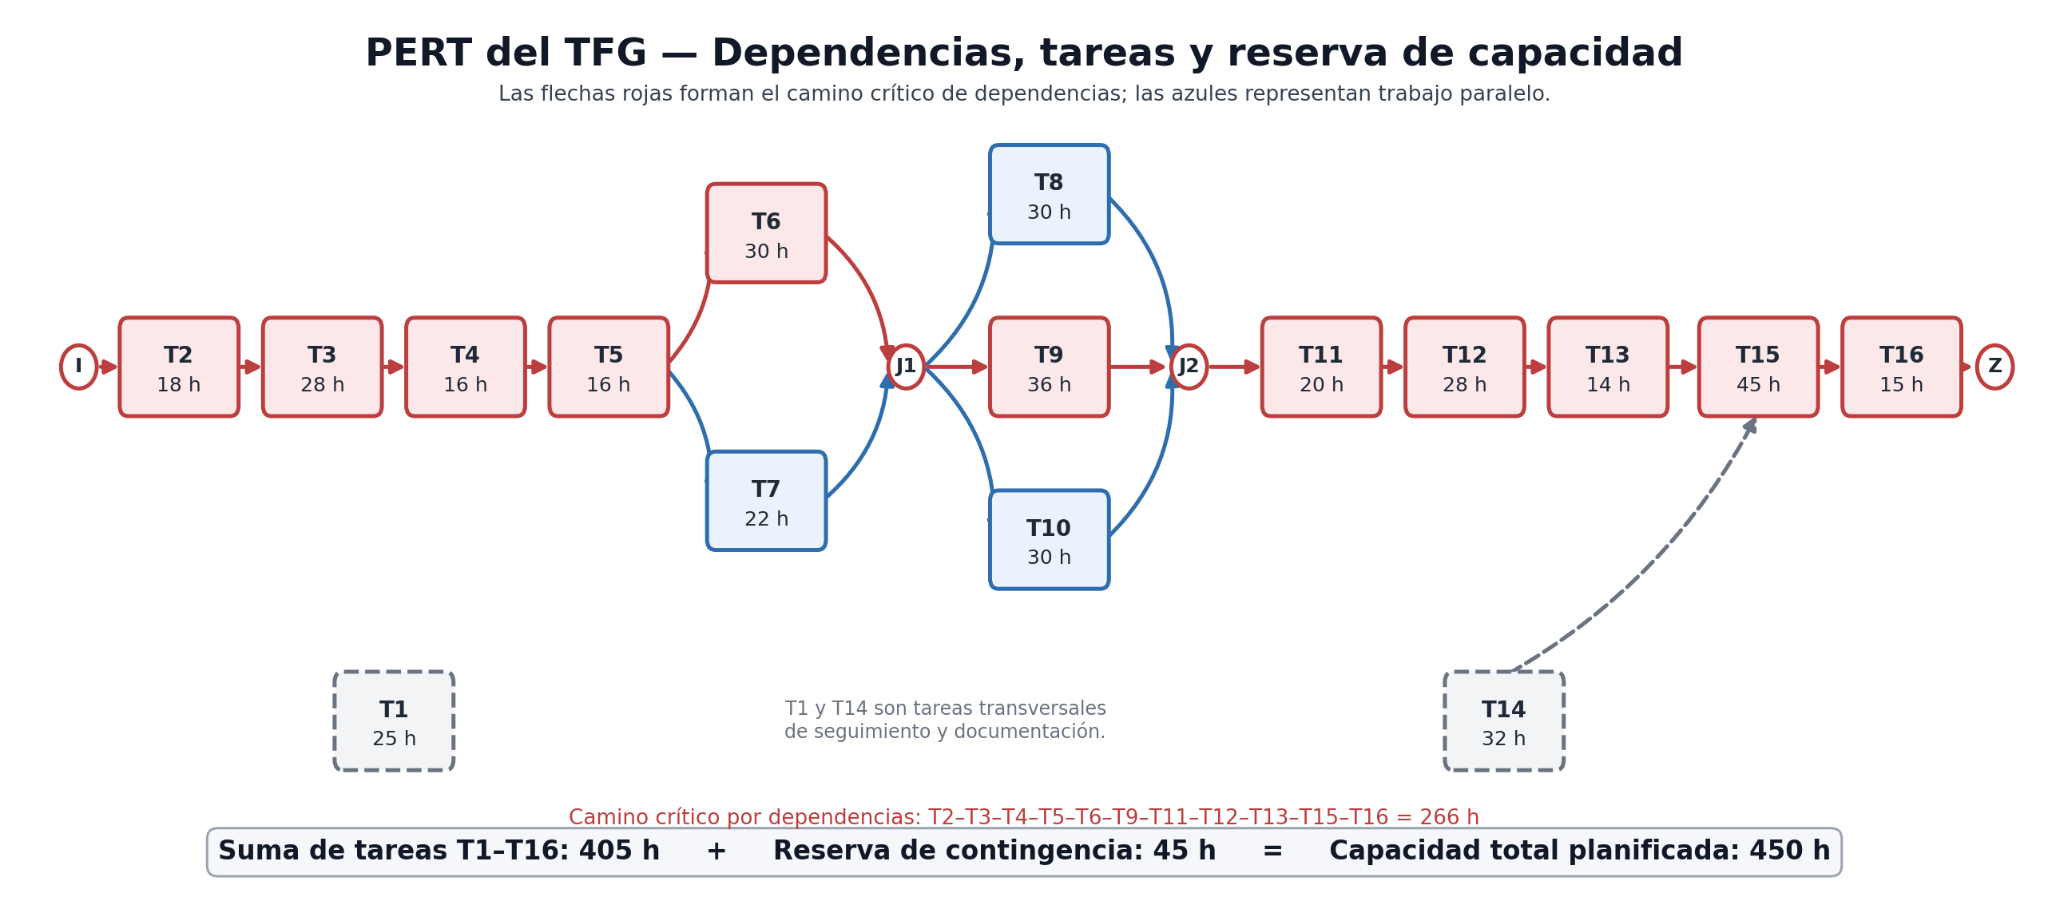
\includegraphics[width=\textwidth]{imagenes/pert.png}
\caption[PERT simplificado y dependencias principales]{PERT simplificado y dependencias principales. La ruta superior representa el camino crítico de referencia}\label{fig:1}
\end{figure}

\needspace{6\baselineskip}
\subsection{Recursos y control de la carga}\label{sec:2-2-3}

El estudiante ejecuta las tareas de análisis, diseño, configuración, desarrollo, pruebas y documentación. La dirección y tutoría aportan contraste metodológico en los hitos; los usuarios de validación revisan la adecuación de los flujos. El entorno de pruebas evita manipular datos reales de menores. Las tareas de mayor esfuerzo son T9, T10 y T15; se han dividido funcionalmente para que el control semanal pueda detectar cualquier desviación.

\needspace{6\baselineskip}
\section{Planificación temporal y diagrama de Gantt}\label{sec:2-3}

El Gantt representa el calendario base de 405 horas y la capacidad de contingencia de 45 horas. Las actividades se ejecutan dentro del intervalo mostrado según las dependencias de las Tablas~\ref{tab:9} y~\ref{tab:10}. Las líneas verticales separan los sprints S1-S4. Gestión y documentación se desarrollan de forma continua; esta concurrencia permite mantener trazabilidad y detectar desviaciones pronto~\cite{ref18,ref20}.

\begin{figure}[htbp]
\centering
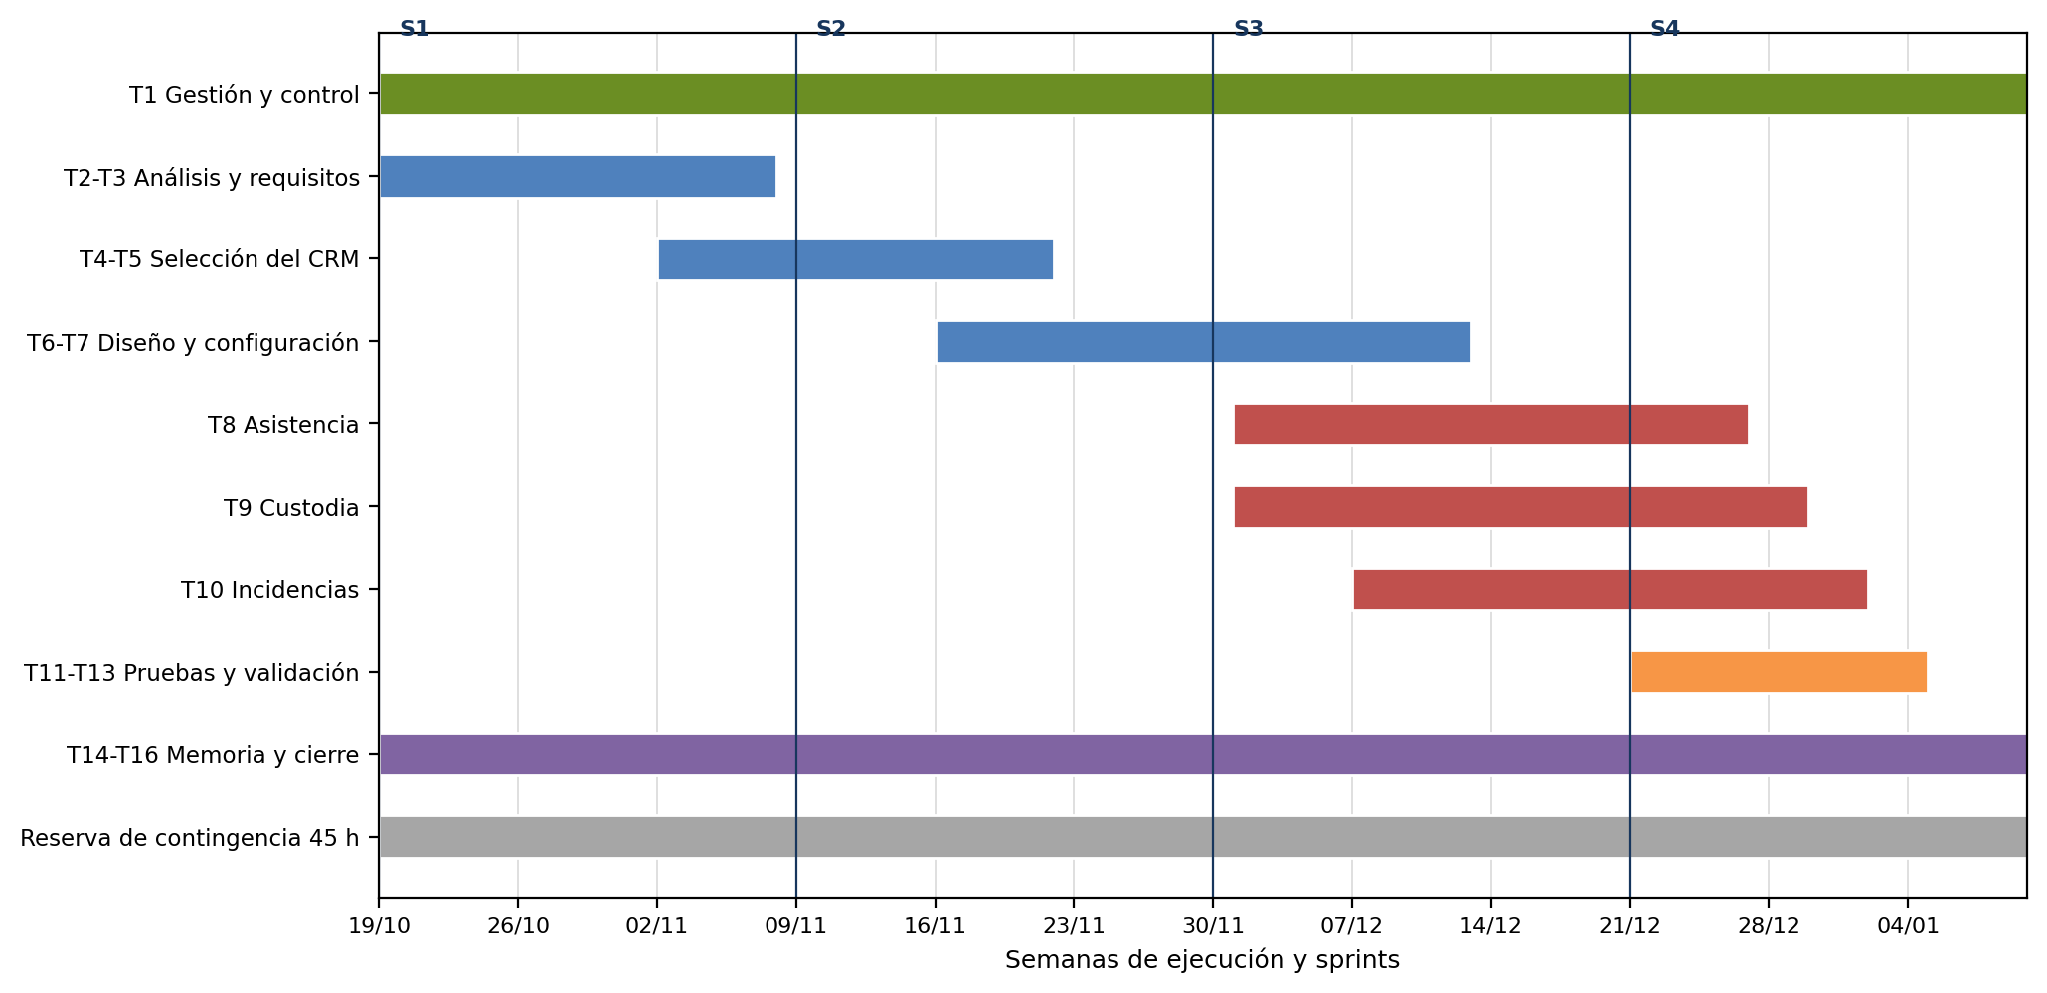
\includegraphics[width=\textwidth]{imagenes/gantt.png}
\caption[Diagrama de Gantt por sprints]{Diagrama de Gantt por sprints. El plan reserva 45 horas de capacidad de contingencia dentro del calendario}\label{fig:2}
\end{figure}

\needspace{12\baselineskip}
\subsection{Hitos de control}\label{sec:2-3-1}

\begin{table}[H]
\centering\small
\begin{tabularx}{\textwidth}{>{\hsize=0.525\hsize\raggedright\arraybackslash}X>{\hsize=1.475\hsize\raggedright\arraybackslash}X}
\toprule
\rowcolor{cabeceratabla} \textbf{Fecha} & \textbf{Resultado verificable} \\
\midrule
H1 · 08/11 & Requisitos y procesos validados \\
H2 · 22/11 & CRM seleccionado y justificado \\
H3 · 13/12 & Modelo, permisos y configuración base listos \\
H4 · 02/01 & Módulos de asistencia, custodia e incidencias adaptados \\
H5 · 05/01 & Pruebas y validación funcional completadas \\
H6 · 10/01 & Memoria cerrada y entrega preparada \\
\bottomrule
\end{tabularx}
\caption{Hitos de control}\label{tab:11}
\end{table}

\needspace{6\baselineskip}
\subsection{Lectura del calendario}\label{sec:2-3-2}

S1 concentra la definición y el contraste del alcance. S2 finaliza la selección y prepara la plataforma. S3 produce los tres módulos prioritarios y comienza las pruebas. S4 cierra la validación, consolida la memoria y deja margen para la revisión final. La carga semanal total es 37,5 horas: 33,75 horas de trabajo base y 3,75 horas no asignadas para contingencias. El periodo navideño se reserva para trabajo individual de construcción y documentación; no se sitúan en él validaciones que dependan de terceros.

\needspace{6\baselineskip}
\subsection{Seguimiento y replanificación}\label{sec:2-3-3}

El Gantt constituye la línea base del proyecto: relaciona tareas, fechas, hitos y dependencias~\cite{ref16,ref17}. La planificación se actualizará con datos reales una vez por semana. No se modificará la fecha final sin evaluar antes el camino crítico, la reserva disponible y los hitos afectados. De este modo se conserva una diferencia visible entre el plan inicial y la ejecución real.

\needspace{6\baselineskip}
\subsection{Indicadores de control por sprint}\label{sec:2-3-4}

Cada revisión semanal compara la situación prevista con la real. Los indicadores no sustituyen al juicio del proyecto, pero permiten decidir si basta con reajustar el orden de trabajo o si es necesario activar una reserva. El avance se comunica en términos de productos verificables, no solo de porcentaje de tiempo consumido.

\begin{table}[H]
\centering\small
\begin{tabularx}{\textwidth}{>{\hsize=1.054\hsize\raggedright\arraybackslash}X>{\hsize=1.404\hsize\raggedright\arraybackslash}X>{\hsize=0.542\hsize\raggedright\arraybackslash}X}
\toprule
\rowcolor{cabeceratabla} \textbf{Indicador} & \textbf{Uso de la información} & \textbf{Frecuencia} \\
\midrule
Horas reales / planificadas & Detectar sobreesfuerzo o subestimación & Semanal \\
Tareas completadas / previstas & Medir cumplimiento del sprint & Semanal \\
Dependencias bloqueadas & Identificar impactos en el camino crítico & Semanal \\
Defectos críticos abiertos & Decidir prioridad de corrección & En pruebas \\
Hitos alcanzados & Confirmar productos verificables & Fin de sprint \\
\bottomrule
\end{tabularx}
\caption{Indicadores de seguimiento}\label{tab:12}
\end{table}

\needspace{12\baselineskip}
\subsection{Cadencia de trabajo}\label{sec:2-3-5}

\begin{table}[H]
\centering\small
\begin{tabularx}{\textwidth}{>{\hsize=0.433\hsize\raggedright\arraybackslash}X>{\hsize=1.567\hsize\raggedright\arraybackslash}X}
\toprule
\rowcolor{cabeceratabla} \textbf{Momento} & \textbf{Actividad de control} \\
\midrule
Lunes & Actualizar el tablero, planificar la semana y priorizar tareas críticas. \\
Mitad de semana & Revisar avance, registrar impedimentos y consultar dudas técnicas. \\
Fin de semana & Comparar horas, actualizar Gantt y preparar evidencia documental. \\
Fin de sprint & Validar el incremento, revisar riesgos y aprobar la siguiente iteración. \\
\bottomrule
\end{tabularx}
\caption{Cadencia de trabajo}\label{tab:13}
\end{table}

Esta cadencia refuerza el carácter iterativo del plan: cada sprint produce un resultado revisable y actualiza las estimaciones de las tareas posteriores sin perder la trazabilidad del calendario base.

\needspace{6\baselineskip}
\section{Gestión de riesgos y planes alternativos}\label{sec:2-4}

Los riesgos se gestionan mediante revisión semanal. Cuando un riesgo se active, se registrará la desviación y se aplicará la respuesta indicada. La reducción de alcance solo se contempla como última medida y nunca afectará a los tres procesos de seguridad infantil: asistencia, custodia e incidencias.

\begin{table}[H]
\centering\footnotesize
\begin{tabularx}{\textwidth}{>{\hsize=0.500\hsize\raggedright\arraybackslash}X>{\hsize=1.195\hsize\raggedright\arraybackslash}X>{\hsize=0.575\hsize\raggedright\arraybackslash}X>{\hsize=1.087\hsize\raggedright\arraybackslash}X>{\hsize=1.643\hsize\raggedright\arraybackslash}X}
\toprule
\rowcolor{cabeceratabla} \textbf{Riesgo} & \textbf{Descripción} & \textbf{Prob. / impacto} & \textbf{Prevención} & \textbf{Plan alternativo} \\
\midrule
R1 & Cambios o ambigüedad en las autorizaciones de recogida & Media / Alta & Prototipo temprano y validación de reglas. & Congelar reglas mínimas y usar 12 h de reserva para adaptar formularios. \\
R2 & Complejidad no prevista al extender SuiteCRM & Media / Alta & Prueba técnica en S2 y módulos pequeños. & Sustituir automatismo no esencial por flujo configurado; reserva de 16 h. \\
R3 & Disponibilidad limitada de usuarios para validar & Alta / Media & Acordar sesiones y casos de prueba con antelación. & Validación asíncrona con guion y evidencia; reserva de 8 h. \\
R4 & Defectos detectados cerca del cierre & Media / Alta & Pruebas por módulo desde S3. & Priorizar defectos críticos y usar 9 h de reserva; mantener H5 como límite. \\
\bottomrule
\end{tabularx}
\caption{Riesgos y respuesta planificada}\label{tab:14}
\end{table}

\needspace{6\baselineskip}
\subsection{Viabilidad del plan alternativo}\label{sec:2-4-1}

La reserva total de 45 horas se distribuye sólo tras comprobar que la desviación amenaza una tarea crítica. Se conserva como capacidad no asignada de 3,75 horas semanales y se utiliza por el estudiante en el entorno local; la directora aprueba cualquier uso superior a ocho horas o que afecte a una regla de seguridad. R1 activa 12 horas si una regla de recogida resulta ambigua o incompatible durante el contraste; R2 activa 16 horas si la prueba técnica impide resolver una personalización crítica; R3 activa 8 horas si no se consigue una sesión de validación; y R4 activa 9 horas si queda un defecto crítico antes de H5. En todos los casos se preservan asistencia, custodia e incidencias. Solo se posponen mejoras no esenciales portal familiar, indicadores ampliados o automatismos no críticos, sin desplazar H5 ni H6.

\needspace{6\baselineskip}
\subsection{Criterio de escalado}\label{sec:2-4-2}

Una desviación de hasta cuatro horas se corrige dentro del sprint y se registra en el seguimiento. Entre cuatro y ocho horas se revisa la secuencia de tareas y se usa la parte de reserva asociada al riesgo. Si supera ocho horas, afecta a la protección de datos o obliga a cambiar una regla de custodia, se consulta a la directora antes de continuar. El alcance se mantiene estable, solo podrían posponerse mejoras de usabilidad, el portal familiar, indicadores ampliados o automatismos no críticos; nunca el control de asistencia, la trazabilidad de custodia ni la gestión de incidencias.


% Generado por trabajo_en_curso/week5/latex/convertir.py a partir del .docx de la memoria.
% A partir de ahora este fichero es la fuente: edítalo directamente.

\chapter{Presupuesto}\label{sec:3}

\needspace{6\baselineskip}
\section{Objeto, criterios y base de cálculo}\label{sec:3-1}

\needspace{6\baselineskip}
\subsection{Hipótesis de trabajo}\label{sec:3-1-1}

El presupuesto global contempla las 540 horas de referencia del TFG. Se compone de 90 horas ya realizadas en las entregas GEP, 405 horas de trabajo base del 19 de octubre de 2026 al 10 de enero de 2027 y 45 horas de contingencia posterior a GEP. Por tanto, se presupuestan tanto las actividades GEP como todas las tareas T1–T16 del Gantt. No se añaden servicios de producción.

El prototipo se ejecutará en el ordenador propio HP Desktop M01-f0xxx, en un entorno local y con datos sintéticos. SuiteCRM, el sistema operativo y las herramientas de desarrollo no requieren licencia de pago para este uso. El presupuesto sí imputa de manera proporcional el equipo, la conectividad, electricidad, copia externa, espacio de trabajo y consumibles. No se incluye despliegue real, mensajería SMS, almacenamiento de datos de menores ni integración con sistemas del centro. Estas decisiones delimitan tanto el coste como los efectos de sostenibilidad.

\needspace{6\baselineskip}
\subsection{Método de estimación}\label{sec:3-1-2}

La estimación es de abajo arriba: a cada tarea del Gantt y a cada actividad GEP se le asignan horas, perfil principal y tarifa imputable. Para no confundir un TFG individual con trabajo gratuito, se usa el coste de perfiles profesionales equivalentes. Las tarifas parten de referencias salariales de Glassdoor y se convierten en coste empresarial aplicando un factor de 1,30 al sueldo bruto por hora para cubrir cotizaciones y costes sociales, siguiendo el criterio del módulo de gestión económica~\cite{ref23,ref24}.

El coste de la reserva de contingencia se mantiene separado de los riesgos identificados. La contingencia cubre variaciones ordinarias de estimación; los imprevistos se calculan como probabilidad por coste del plan B. No se añade IVA: el resultado es un coste interno de proyecto, no un presupuesto comercial.

\needspace{6\baselineskip}
\section{Presupuesto del proyecto}\label{sec:3-2}

\needspace{6\baselineskip}
\subsection{Costes de personal y criterio salarial}\label{sec:3-2-1}

Se consideran cinco perfiles equivalentes, aunque una sola persona pueda asumirlos en el contexto académico. La distinción permite valorar adecuadamente la naturaleza de cada actividad y facilita el seguimiento por tipo de trabajo. Las referencias salariales se consultaron el 2 de octubre de 2026; se toma una jornada anual de 1.760 horas para convertir el salario anual en coste bruto horario.

\begin{table}[H]
\centering\footnotesize
\begin{tabularx}{\textwidth}{>{\hsize=1.138\hsize\raggedright\arraybackslash}X>{\hsize=1.621\hsize\raggedright\arraybackslash}X>{\hsize=0.526\hsize\raggedright\arraybackslash}X>{\hsize=0.619\hsize\raggedright\arraybackslash}X>{\hsize=0.896\hsize\raggedright\arraybackslash}X>{\hsize=1.221\hsize\raggedright\arraybackslash}X}
\toprule
\rowcolor{cabeceratabla} \textbf{Perfil equivalente} & \textbf{Referencia salarial} & \textbf{Bruto €/h} & \textbf{Factor} & \textbf{Tarifa imputable €/h} & \textbf{Uso principal} \\
\midrule
Coordinación del proyecto & Technical Project Manager, Barcelona: 22 €/h~\cite{ref25} & 22,00 & $\times$ 1,30 & 28,60 & Planificación, control y cierre \\
Análisis funcional & Referencia conservadora entre perfiles TIC junior de Glassdoor~\cite{ref26} & 16,50 & $\times$ 1,30 & 21,45 & Procesos, requisitos, datos y selección \\
Desarrollo CRM & Salesforce Developer, Barcelona: 18 €/h~\cite{ref27} & 18,00 & $\times$ 1,30 & 23,40 & Configuración y extensiones SuiteCRM \\
Pruebas & QA Automation Tester, España: 13 €/h~\cite{ref28} & 13,00 & $\times$ 1,30 & 16,90 & Casos de prueba y validación \\
Documentación técnica & Tarifa equivalente a perfil TIC junior~\cite{ref26} & 16,00 & $\times$ 1,30 & 20,80 & Memoria, anexos y guía de uso \\
\bottomrule
\end{tabularx}
\caption{Perfiles y tarifas imputables}\label{tab:15}
\end{table}

La tarifa de análisis funcional y documentación se sitúa deliberadamente en un nivel junior y se justifica por la naturaleza académica del prototipo. No se utiliza el precio por hora de una consultora, que incluiría margen comercial y no refleja el coste interno requerido por esta entrega.

\needspace{6\baselineskip}
\subsection{Coste directo por tarea del Gantt}\label{sec:3-2-2}

Las tablas siguientes establecen la trazabilidad entre las actividades GEP, la planificación del GEP 2 y el presupuesto. Cada actividad se asigna a un único perfil predominante para evitar doble contabilización. Las horas base suman 495; las 45 horas de reserva posterior a GEP se muestran posteriormente como partida independiente.

\begin{table}[H]
\centering\footnotesize
\begin{tabularx}{\textwidth}{>{\hsize=0.477\hsize\raggedright\arraybackslash}X>{\hsize=2.472\hsize\raggedright\arraybackslash}X>{\hsize=1.057\hsize\raggedright\arraybackslash}X>{\hsize=0.526\hsize\raggedright\arraybackslash}X>{\hsize=0.676\hsize\raggedright\arraybackslash}X>{\hsize=0.791\hsize\raggedright\arraybackslash}X}
\toprule
\rowcolor{cabeceratabla} \textbf{ID} & \textbf{Actividad planificada} & \textbf{Perfil} & \textbf{Horas} & \textbf{€/h} & \textbf{Coste} \\
\midrule
T1 & Planificación y seguimiento & Coordinación & 25 & 28,60 & 715,00 \\
T2 & Actores y casos de uso & Análisis & 18 & 21,45 & 386,10 \\
T3 & Proceso, requisitos y protección de datos & Análisis & 28 & 21,45 & 600,60 \\
T4 & Criterios, preselección y POC & Análisis & 16 & 21,45 & 343,20 \\
T5 & Comparativa y selección CRM & Análisis & 16 & 21,45 & 343,20 \\
T6 & Datos, roles y trazabilidad & Análisis & 30 & 21,45 & 643,50 \\
T7 & Entorno y configuración base & Desarrollo & 22 & 23,40 & 514,80 \\
T8 & Módulo de asistencia & Desarrollo & 30 & 23,40 & 702,00 \\
\bottomrule
\end{tabularx}
\caption{Coste directo por tarea del Gantt (parte 1)}\label{tab:16}
\end{table}

\begin{table}[H]
\centering\footnotesize
\begin{tabularx}{\textwidth}{>{\hsize=0.482\hsize\raggedright\arraybackslash}X>{\hsize=2.401\hsize\raggedright\arraybackslash}X>{\hsize=1.138\hsize\raggedright\arraybackslash}X>{\hsize=0.526\hsize\raggedright\arraybackslash}X>{\hsize=0.632\hsize\raggedright\arraybackslash}X>{\hsize=0.821\hsize\raggedright\arraybackslash}X}
\toprule
\rowcolor{cabeceratabla} \textbf{ID} & \textbf{Actividad planificada} & \textbf{Perfil} & \textbf{Horas} & \textbf{€/h} & \textbf{Coste} \\
\midrule
T9 & Custodia y autorizaciones & Desarrollo & 36 & 23,40 & 842,40 \\
T10 & Incidencias, prioridad y escalado & Desarrollo & 30 & 23,40 & 702,00 \\
T11 & Diseño de pruebas y datos sintéticos & Pruebas & 20 & 16,90 & 338,00 \\
T12 & Ejecución de pruebas y correcciones & Pruebas & 28 & 16,90 & 473,20 \\
T13 & Validación funcional & Pruebas & 14 & 16,90 & 236,60 \\
T14 & Documentación continua & Documentación & 32 & 20,80 & 665,60 \\
T15 & Memoria, anexos y guía & Documentación & 45 & 20,80 & 936,00 \\
T16 & Revisión, entrega y defensa & Documentación & 15 & 20,80 & 312,00 \\
 & TOTAL POST-GEP &  & 405 &  & 8.754,20 \\
\bottomrule
\end{tabularx}
\caption{Coste directo por tarea del Gantt (parte 2)}\label{tab:17}
\end{table}

El coste directo posterior a GEP es 8.754,20 €. Las actividades GEP ya realizadas se incorporan de forma retrospectiva para reflejar las 540 horas completas del TFG. El coste directo total asciende a 10.879,70 €. El mayor esfuerzo posterior a GEP corresponde al desarrollo de los tres módulos (2.761,20 €) y al análisis, procesos y decisión de CRM (2.316,60 €), coherente con un producto que configura procesos sensibles de menores y sus controles.

\begin{table}[H]
\centering\footnotesize
\begin{tabularx}{\textwidth}{>{\hsize=0.469\hsize\raggedright\arraybackslash}X>{\hsize=2.473\hsize\raggedright\arraybackslash}X>{\hsize=1.138\hsize\raggedright\arraybackslash}X>{\hsize=0.526\hsize\raggedright\arraybackslash}X>{\hsize=0.476\hsize\raggedright\arraybackslash}X>{\hsize=0.918\hsize\raggedright\arraybackslash}X}
\toprule
\rowcolor{cabeceratabla} \textbf{ID} & \textbf{Actividad ya realizada} & \textbf{Perfil} & \textbf{Horas} & \textbf{€/h} & \textbf{Coste (€)} \\
\midrule
GEP1 & Contexto, alcance y selección & Análisis funcional & 30 & 21,45 & 643,50 \\
GEP2 & Planificación, Gantt y riesgos & Coordinación & 30 & 28,60 & 858,00 \\
GEP3 & Presupuesto, control y sostenibilidad & Documentación técnica & 30 & 20,80 & 624,00 \\
 & TOTAL ACTIVIDADES GEP &  & 90 &  & 2.125,50 \\
 & TOTAL COSTE DIRECTO GLOBAL &  & 495 &  & 10.879,70 \\
\bottomrule
\end{tabularx}
\caption{Coste de las actividades GEP y coste directo global}\label{tab:18}
\end{table}

\needspace{6\baselineskip}
\subsection{Costes generales del prototipo}\label{sec:3-2-3}

Los costes generales recogen recursos que no se asignan a una tarea concreta. El equipo se amortiza linealmente durante cuatro años, de forma proporcional a las 495 horas base del TFG. También se imputan de manera conservadora la conectividad, electricidad, copia externa, espacio de trabajo y consumibles. El software tiene coste de licencia nulo al usarse soluciones libres o ya disponibles; ello no elimina el esfuerzo de configuración, que ya figura como coste de personal.

\begin{table}[H]
\centering\small
\begin{tabularx}{\textwidth}{>{\hsize=1.157\hsize\raggedright\arraybackslash}X>{\hsize=1.400\hsize\raggedright\arraybackslash}X>{\hsize=0.443\hsize\raggedright\arraybackslash}X}
\toprule
\rowcolor{cabeceratabla} \textbf{Concepto} & \textbf{Cálculo} & \textbf{Coste (€)} \\
\midrule
Ordenador (amortización) & 900 € / (4 años $\times$ 1.760 h) $\times$ 495 h & 63,28 \\
Conectividad doméstica & 20 €/mes $\times$ 4 meses & 80,00 \\
Electricidad & 0,060 kW $\times$ 495 h $\times$ 0,2074 €/kWh~\cite{ref29} & 6,16 \\
Copia de seguridad externa & 5 €/mes $\times$ 4 meses & 20,00 \\
Licencias SuiteCRM y herramientas & Software libre / herramientas ya disponibles & 0,00 \\
Espacio de trabajo & 25 €/mes $\times$ 4 meses (imputación proporcional) & 100,00 \\
Consumibles & Estimación fija del periodo & 10,00 \\
TOTAL COSTES GENERALES &  & 279,44 \\
\bottomrule
\end{tabularx}
\caption{Costes generales del prototipo}\label{tab:19}
\end{table}

La reserva de contingencia mantiene 45 horas, pues corresponde al trabajo posterior a GEP todavía pendiente. Equivale al 11,1 \% de las 405 horas posteriores a GEP y al 9,1 \% de las 495 horas base globales. Para valorarla se aplica el coste medio ponderado del personal de todo el TFG: 10.879,70 € / 495 h = 21,98 €/h. Esta reserva se sitúa dentro de la recomendación habitual del 10–20 \% para proyectos informáticos~\cite{ref23}.

\begin{table}[H]
\centering\small
\begin{tabularx}{\textwidth}{>{\hsize=1.263\hsize\raggedright\arraybackslash}X>{\hsize=1.301\hsize\raggedright\arraybackslash}X>{\hsize=0.437\hsize\raggedright\arraybackslash}X}
\toprule
\rowcolor{cabeceratabla} \textbf{Partida} & \textbf{Base de cálculo} & \textbf{Coste (€)} \\
\midrule
Contingencia genérica & 45 h $\times$ 21,98 €/h & 989,10 \\
R1. Ajuste de requisitos & 30 \% $\times$ (12 h de análisis $\times$ 21,45 €/h) & 77,22 \\
R2. Complejidad de personalización & 35 \% $\times$ (16 h de desarrollo $\times$ 23,40 €/h) & 131,04 \\
R3. Repetición de pruebas & 45 \% $\times$ (8 h de pruebas $\times$ 16,90 €/h) & 60,84 \\
R4. Correcciones de documentación & 40 \% $\times$ (9 h de desarrollo $\times$ 23,40 €/h) & 84,24 \\
TOTAL IMPREVISTOS ESPECÍFICOS &  & 353,34 \\
\bottomrule
\end{tabularx}
\caption{Contingencia e imprevistos específicos}\label{tab:20}
\end{table}

Los riesgos R1–R4 proceden del registro de riesgos y de los planes B asociados al GEP 2. Su importe no se suma a las horas de trabajo planificadas: se trata de una provisión esperada que solo se consumiría si se materializa el evento. Antes de usarla se revisará que no pueda absorberse con la contingencia general.

\needspace{11\baselineskip}
\subsection{Resumen presupuestario}\label{sec:3-2-4}

\begin{table}[H]
\centering\small
\begin{tabularx}{\textwidth}{>{\hsize=1.477\hsize\raggedright\arraybackslash}X>{\hsize=0.817\hsize\raggedright\arraybackslash}X>{\hsize=0.706\hsize\raggedright\arraybackslash}X}
\toprule
\rowcolor{cabeceratabla} \textbf{Bloque} & \textbf{Coste (€)} & \textbf{Peso} \\
\midrule
Personal directo & 10.879,70 & 87,03 \% \\
Costes generales & 279,44 & 2,24 \% \\
Contingencia genérica & 989,10 & 7,91 \% \\
Imprevistos específicos & 353,34 & 2,83 \% \\
TOTAL PRESUPUESTO & 12.501,58 & 100,00 \% \\
\bottomrule
\end{tabularx}
\caption{Resumen presupuestario global}\label{tab:21}
\end{table}

El presupuesto global asciende a 12.501,58 €. La cifra incorpora las 540 horas de referencia del TFG y permite valorar la viabilidad del alcance como coste profesional equivalente. Para un centro escolar, una adopción real requeriría un presupuesto adicional de producción —hosting, soporte, formación, evaluación de protección de datos e integración— que queda expresamente fuera del TFG.

\needspace{6\baselineskip}
\section{Seguimiento y control económico}\label{sec:3-3}

El control se realizará semanalmente junto con la actualización del Gantt. Cada viernes registraré horas reales, coste real, tareas completadas, consumo de reserva y cambios en riesgos. El registro separará coste directo, costes generales, contingencia e imprevistos para que una desviación no quede oculta dentro del total.

\begin{table}[H]
\centering\small
\begin{tabularx}{\textwidth}{>{\hsize=0.819\hsize\raggedright\arraybackslash}X>{\hsize=1.043\hsize\raggedright\arraybackslash}X>{\hsize=1.138\hsize\raggedright\arraybackslash}X}
\toprule
\rowcolor{cabeceratabla} \textbf{Indicador} & \textbf{Fórmula} & \textbf{Umbral y acción} \\
\midrule
Coste planificado (CP) & $\Sigma$ horas planificadas ejecutadas $\times$ tarifa & Referencia de cada semana \\
Coste real (CR) & $\Sigma$ horas reales $\times$ tarifa + gastos reales & Se actualiza semanalmente \\
Desviación absoluta & CR $-$ CP & Amarillo: \textgreater{} 5 \% del CP; rojo: \textgreater{} 10 \% \\
Desviación porcentual & (CR $-$ CP) / CP $\times$ 100 & Analizar causa y estimar cierre \\
Consumo de contingencia & Horas de reserva usadas / 45 h & Revisión obligatoria al superar 50 \% \\
Riesgo esperado pendiente & $\Sigma$ probabilidad $\times$ coste plan B & Actualizar al cambiar probabilidad \\
Previsión a término & CR acumulado + coste pendiente estimado & No superar 12.501,58 € sin decisión \\
\bottomrule
\end{tabularx}
\caption{Indicadores de control económico}\label{tab:22}
\end{table}

\needspace{6\baselineskip}
\subsection{Mecanismo de decisión}\label{sec:3-3-1}

Una desviación inferior al 5 \% se documentará sin modificar la línea base. Entre el 5 \% y el 10 \% revisaré la estimación de las tareas pendientes y priorizaré entregables del alcance mínimo. Si la previsión supera el 10 \% o se consume más de la mitad de la contingencia antes de T12, prepararé una propuesta de reajuste para la directora: reasignar horas, reducir trabajo no esencial o aprobar el uso de una partida de imprevistos. Ninguna partida de riesgo se utilizará para trabajo ordinario.

\needspace{6\baselineskip}
\subsection{Evidencias de control}\label{sec:3-3-2}

Conservaré una hoja de cálculo de control con fecha, tarea, horas previstas y reales, perfil, coste, incidencia, decisión y responsable. Junto a ella, el Gantt actualizado y el registro de riesgos permitirán explicar la variación entre presupuesto y ejecución. Al cierre, compararé coste final, coste previsto y reserva consumida para evaluar la calidad de la estimación.


% Generado por trabajo_en_curso/week5/latex/convertir.py a partir del .docx de la memoria.
% A partir de ahora este fichero es la fuente: edítalo directamente.

\chapter{Especificación}\label{sec:4}

Este apartado especifica el producto mínimo del TFG para la gestión segura de actividades extraescolares de primaria. Toma como línea base los requisitos del apartado~\ref{sec:1-3-4} y concreta el comportamiento del sistema mediante casos de uso~\cite{ref36}, un modelo conceptual en UML~\cite{ref35}, restricciones de integridad en OCL~\cite{ref34}, plantillas Volere para los requisitos no funcionales~\cite{ref37}, historias de usuario~\cite{ref38} y pruebas. Todos los ejemplos de validación usan datos sintéticos.

La especificación cubre la información de alumnos, contactos y autorizaciones; la preparación de sesiones; el registro de asistencia; la custodia y entrega; la gestión y comunicación de incidencias; y la consulta de historial con control de permisos. RF08 y RF09 se mantienen como incrementos posteriores: intercambio CSV autorizado, indicadores agregados y un portal familiar limitado.

\begin{table}[H]
\centering\small
\begin{tabularx}{\textwidth}{>{\hsize=0.487\hsize\raggedright\arraybackslash}X>{\hsize=1.513\hsize\raggedright\arraybackslash}X}
\toprule
\rowcolor{cabeceratabla} \textbf{Elemento} & \textbf{Tratamiento en la especificación} \\
\midrule
Requisitos funcionales & Se detallan en casos de uso, historias de usuario, modelo conceptual y restricciones OCL. \\
Requisitos no funcionales & Se detallan mediante fichas Volere con criterio de aceptación y método de evaluación. \\
Validación & Se define una evidencia por requisito con escenarios sintéticos y perfiles incompatibles. \\
\bottomrule
\end{tabularx}
\caption{Enfoque de especificación}\label{tab:23}
\end{table}

\needspace{6\baselineskip}
\section{Modelo de casos de uso}\label{sec:4-1}

El modelo recoge los actores operativos del centro. Administración prepara los datos de alumnos e inscripciones; el monitor registra los hechos de la sesión; coordinación resuelve excepciones, incidencias y comunicaciones; y dirección consulta únicamente la información escalada o agregada. La familia participa como destinataria autorizada de comunicaciones y como fuente de actualización de autorizaciones, sin acceso a información ajena.

\begin{figure}[htbp]
\centering
\figurapendiente{Insertar aquí la Figura 3: diagrama de casos de uso}
\caption{Diagrama de casos de uso del sistema}\label{fig:3}
\end{figure}

Los casos de uso se han agrupado de manera que cada requisito funcional obligatorio queda cubierto al menos una vez. La gestión de autorización prepara el control de custodia; la sesión genera la lista de asistencia; y una incidencia puede desencadenar una comunicación controlada.

\needspace{14\baselineskip}
\subsection{Casos de uso, actores y requisitos cubiertos}\label{sec:4-1-1}

\begin{table}[H]
\centering\small
\begin{tabularx}{\textwidth}{>{\hsize=0.420\hsize\raggedright\arraybackslash}X>{\hsize=1.635\hsize\raggedright\arraybackslash}X>{\hsize=1.246\hsize\raggedright\arraybackslash}X>{\hsize=0.700\hsize\raggedright\arraybackslash}X}
\toprule
\rowcolor{cabeceratabla} \textbf{ID} & \textbf{Caso de uso} & \textbf{Actor principal} & \textbf{Requisitos} \\
\midrule
CU01 & Gestionar ficha y autorizaciones & Administración / coordinación & RF01 \\
CU02 & Preparar sesión y lista & Coordinación & RF02 \\
CU03 & Registrar asistencia & Monitor & RF03 \\
CU04 & Registrar entrega y custodia & Monitor & RF04 \\
CU05 & Gestionar incidencia & Monitor / coordinación & RF05 \\
CU06 & Comunicar incidencia & Coordinación & RF06 \\
CU07 & Consultar historial autorizado & Coordinación / dirección & RF07 \\
\bottomrule
\end{tabularx}
\caption{Casos de uso, actores y requisitos funcionales que cubren}\label{tab:24}
\end{table}

\needspace{6\baselineskip}
\subsection{Descripción de los casos de uso}\label{sec:4-1-2}

Cada caso de uso se describe con una ficha~\cite{ref36}. Las extensiones representan alternativas o errores que se apartan del flujo principal y se identifican con el número del paso al que sustituyen. Los flujos no sustituyen las reglas de autorización, que se verifican además con las restricciones OCL y las pruebas del apartado~\ref{sec:4-5}.

\needspace{22\baselineskip}
\subsubsection{CU01 Gestionar ficha y autorizaciones}\label{sec:4-1-2-1}

\begin{table}[H]
\centering\small
\begin{tabularx}{\textwidth}{>{\hsize=0.381\hsize\raggedright\arraybackslash}X>{\hsize=1.619\hsize\raggedright\arraybackslash}X}
\toprule
\rowcolor{cabeceratabla} \textbf{Campo} & \textbf{Especificación} \\
\midrule
Actor principal & Administración \\
Actor secundario & Coordinación; familia como origen de la información \\
Precondición & El usuario dispone de permiso sobre el alumno o se trata de un alta nueva. \\
Flujo principal & 1. El usuario crea o localiza la ficha del alumno. \newline 2. Registra o actualiza los contactos responsables. \newline 3. Registra la inscripción en una actividad y su estado. \newline 4. Añade una autorización de recogida con fechas de vigencia y estado. \newline 5. El sistema valida los campos obligatorios y guarda el cambio con autor y fecha. \\
Extensiones & 4a. La fecha final es anterior a la inicial: el sistema informa del error y no guarda la autorización. \newline 5a. Falta identificador, nombre o contacto responsable: el sistema impide guardar la ficha. \\
Postcondición & La ficha queda disponible para sesiones futuras; solo las autorizaciones activas y vigentes pueden usarse en una entrega. \\
Requisitos & RF01, RNF01 \\
\bottomrule
\end{tabularx}
\caption{Ficha del caso de uso CU01}\label{tab:25}
\end{table}

\needspace{21\baselineskip}
\subsubsection{CU02 Preparar sesión y lista}\label{sec:4-1-2-2}

\begin{table}[H]
\centering\small
\begin{tabularx}{\textwidth}{>{\hsize=0.387\hsize\raggedright\arraybackslash}X>{\hsize=1.613\hsize\raggedright\arraybackslash}X}
\toprule
\rowcolor{cabeceratabla} \textbf{Campo} & \textbf{Especificación} \\
\midrule
Actor principal & Coordinación \\
Actor secundario & Monitor \\
Precondición & La actividad, el grupo y las inscripciones existen y están actualizados. \\
Flujo principal & 1. La coordinación selecciona actividad y grupo. \newline 2. Crea la sesión con fecha, hora de inicio y fin. \newline 3. El sistema valida que el inicio sea anterior al fin. \newline 4. El sistema genera la lista desde las inscripciones activas de la actividad. \newline 5. La coordinación publica la sesión para el monitor asignado. \\
Extensiones & 3a. El intervalo de la sesión no es válido: el sistema no permite crearla. \newline 4a. Una inscripción está cancelada o pertenece a otra actividad: no se incorpora a la lista. \\
Postcondición & La sesión queda preparada con una lista coherente de alumnos previstos. \\
Requisitos & RF02, RNF01 \\
\bottomrule
\end{tabularx}
\caption{Ficha del caso de uso CU02}\label{tab:26}
\end{table}

\needspace{21\baselineskip}
\subsubsection{CU03 Registrar asistencia}\label{sec:4-1-2-3}

\begin{table}[H]
\centering\small
\begin{tabularx}{\textwidth}{>{\hsize=0.381\hsize\raggedright\arraybackslash}X>{\hsize=1.619\hsize\raggedright\arraybackslash}X}
\toprule
\rowcolor{cabeceratabla} \textbf{Campo} & \textbf{Especificación} \\
\midrule
Actor principal & Monitor \\
Actor secundario & Coordinación \\
Precondición & Existe una sesión publicada, el monitor está asignado y el alumno figura en la lista. \\
Flujo principal & 1. El monitor abre la sesión. \newline 2. Selecciona el estado de cada alumno: presente, ausente, retraso o ausencia justificada. \newline 3. Añade motivo cuando el estado lo requiere. \newline 4. El sistema registra hora y usuario. \newline 5. El monitor confirma el resumen de la sesión. \\
Extensiones & 2a. Ya existe un registro para el mismo alumno y sesión: el sistema muestra el registro existente y permite una corrección trazable. \newline 3a. El estado requiere motivo y este falta: el sistema solicita completarlo. \\
Postcondición & Cada alumno de la lista tiene un estado controlado y no hay duplicados activos para la misma sesión. \\
Requisitos & RF03, RNF01, RNF03 \\
\bottomrule
\end{tabularx}
\caption{Ficha del caso de uso CU03}\label{tab:27}
\end{table}

\needspace{22\baselineskip}
\subsubsection{CU04 Registrar entrega y custodia}\label{sec:4-1-2-4}

\begin{table}[H]
\centering\small
\begin{tabularx}{\textwidth}{>{\hsize=0.381\hsize\raggedright\arraybackslash}X>{\hsize=1.619\hsize\raggedright\arraybackslash}X}
\toprule
\rowcolor{cabeceratabla} \textbf{Campo} & \textbf{Especificación} \\
\midrule
Actor principal & Monitor \\
Actor secundario & Coordinación; persona autorizada \\
Precondición & La sesión ha finalizado o está en fase de entrega; el alumno figura como presente o requiere revisión. \\
Flujo principal & 1. El monitor selecciona al alumno pendiente de entrega. \newline 2. Selecciona o identifica a la persona receptora. \newline 3. El sistema consulta una autorización activa y vigente para ese alumno. \newline 4. Comprueba que no existe otra entrega confirmada. \newline 5. Registra hora, responsable y resultado de la entrega. \newline 6. Muestra confirmación al monitor. \\
Extensiones & 3a. La persona no está autorizada o la autorización está vencida: el sistema bloquea la entrega y registra la excepción. \newline 4a. Ya existe una entrega confirmada: el sistema impide una segunda confirmación y muestra el historial. \\
Postcondición & La entrega autorizada queda asociada a alumno, sesión, receptor y responsable; una excepción queda escalada. \\
Requisitos & RF04, RNF01, RNF03 \\
\bottomrule
\end{tabularx}
\caption{Ficha del caso de uso CU04}\label{tab:28}
\end{table}

\needspace{22\baselineskip}
\subsubsection{CU05 Gestionar incidencia}\label{sec:4-1-2-5}

\begin{table}[H]
\centering\small
\begin{tabularx}{\textwidth}{>{\hsize=0.381\hsize\raggedright\arraybackslash}X>{\hsize=1.619\hsize\raggedright\arraybackslash}X}
\toprule
\rowcolor{cabeceratabla} \textbf{Campo} & \textbf{Especificación} \\
\midrule
Actor principal & Monitor \\
Actor secundario & Coordinación; dirección si se escala \\
Precondición & El usuario pertenece al ámbito de la actividad o sesión relacionada. \\
Flujo principal & 1. El usuario abre una incidencia y selecciona tipo y prioridad. \newline 2. Describe el hecho de forma objetiva y lo vincula a alumno o sesión cuando procede. \newline 3. El sistema asigna estado inicial y conserva autor y fecha. \newline 4. Coordinación asigna responsable y registra la actuación o el escalado. \newline 5. Coordinación cierra la incidencia cuando la actuación está documentada. \\
Extensiones & 2a. Falta la información mínima: el sistema solicita completar tipo, prioridad y descripción. \newline 5a. No existe responsable o actuación: el sistema no permite cerrar la incidencia. \\
Postcondición & La incidencia mantiene su secuencia de estados, responsables y actuaciones. \\
Requisitos & RF05, RNF01 \\
\bottomrule
\end{tabularx}
\caption{Ficha del caso de uso CU05}\label{tab:29}
\end{table}

\needspace{21\baselineskip}
\subsubsection{CU06 Comunicar incidencia}\label{sec:4-1-2-6}

\begin{table}[H]
\centering\small
\begin{tabularx}{\textwidth}{>{\hsize=0.381\hsize\raggedright\arraybackslash}X>{\hsize=1.619\hsize\raggedright\arraybackslash}X}
\toprule
\rowcolor{cabeceratabla} \textbf{Campo} & \textbf{Especificación} \\
\midrule
Actor principal & Coordinación \\
Actor secundario & Familia o persona autorizada \\
Precondición & Existe una incidencia registrada y la coordinación tiene permiso para decidir la comunicación. \\
Flujo principal & 1. Coordinación revisa prioridad, actuaciones y destinatarios posibles. \newline 2. Selecciona el destinatario autorizado y el canal permitido. \newline 3. Redacta o valida el mensaje con la información necesaria. \newline 4. El sistema registra el envío, la fecha y el usuario responsable. \newline 5. Registra el acuse cuando se recibe. \\
Extensiones & 2a. El destinatario no está vinculado o autorizado: el sistema impide el envío. \newline 3a. El mensaje contiene datos fuera del ámbito: la coordinación debe revisarlo antes de confirmar. \\
Postcondición & La comunicación queda vinculada a la incidencia y a un destinatario identificable. \\
Requisitos & RF06, RNF01 \\
\bottomrule
\end{tabularx}
\caption{Ficha del caso de uso CU06}\label{tab:30}
\end{table}

\needspace{24\baselineskip}
\subsubsection{CU07 Consultar historial autorizado}\label{sec:4-1-2-7}

\begin{table}[H]
\centering\small
\begin{tabularx}{\textwidth}{>{\hsize=0.381\hsize\raggedright\arraybackslash}X>{\hsize=1.619\hsize\raggedright\arraybackslash}X}
\toprule
\rowcolor{cabeceratabla} \textbf{Campo} & \textbf{Especificación} \\
\midrule
Actor principal & Coordinación \\
Actor secundario & Dirección \\
Precondición & El usuario ha iniciado sesión y posee rol y ámbito configurados. \\
Flujo principal & 1. El usuario busca un alumno, sesión o incidencia dentro de su ámbito. \newline 2. El sistema comprueba el rol, la actividad y la finalidad de consulta. \newline 3. Recupera la secuencia de asistencia, custodia, incidencias y comunicaciones permitidas. \newline 4. El usuario consulta el detalle o solicita una exportación autorizada. \newline 5. El sistema conserva la acción de consulta o exportación en la auditoría. \\
Extensiones & 2a. El usuario intenta acceder a un grupo ajeno: el sistema deniega el acceso. \newline 4a. La exportación contiene datos innecesarios: el sistema limita los campos al ámbito autorizado. \\
Postcondición & El historial se muestra ordenado temporalmente y sin exponer datos ajenos. \\
Requisitos & RF07, RNF01 \\
\bottomrule
\end{tabularx}
\caption{Ficha del caso de uso CU07}\label{tab:31}
\end{table}

\needspace{6\baselineskip}
\section{Modelo conceptual y restricciones de integridad}\label{sec:4-2}

El modelo conceptual identifica la información mínima que debe configurarse o extenderse en el CRM. El alumno es la entidad protegida; las autorizaciones, inscripciones y eventos se vinculan a él para poder reconstruir el historial de cada sesión sin depender de conversaciones privadas o listas duplicadas.

\begin{figure}[htbp]
\centering
\figurapendiente{Insertar aquí la Figura 4: modelo conceptual}
\caption{Modelo conceptual de asistencia, custodia e incidencias}\label{fig:4}
\end{figure}

\needspace{19\baselineskip}
\subsection{Diccionario de entidades}\label{sec:4-2-1}

\begin{table}[H]
\centering\small
\begin{tabularx}{\textwidth}{>{\hsize=0.673\hsize\raggedright\arraybackslash}X>{\hsize=1.294\hsize\raggedright\arraybackslash}X>{\hsize=1.033\hsize\raggedright\arraybackslash}X}
\toprule
\rowcolor{cabeceratabla} \textbf{Entidad} & \textbf{Responsabilidad} & \textbf{Atributos críticos} \\
\midrule
Alumno & Sujeto protegido al que se asocian inscripciones y eventos. & Identificador, nombre, fecha de nacimiento. \\
Autorización & Vincula alumno y contacto durante un periodo. & Estado, fecha inicial y fecha final. \\
Sesión & Representa una instancia concreta de una actividad. & Inicio, fin, estado, grupo. \\
Asistencia & Registra el estado del alumno en una sesión. & Estado, hora, autor, motivo. \\
EntregaCustodia & Conserva evidencia de una entrega o excepción. & Hora, resultado, receptor, responsable. \\
Incidencia & Gestiona un hecho relevante y sus actuaciones. & Tipo, prioridad, estado, responsable. \\
Comunicación & Registra los avisos vinculados a una incidencia. & Canal, destinatario, envío, acuse. \\
\bottomrule
\end{tabularx}
\caption{Diccionario de entidades}\label{tab:32}
\end{table}

\needspace{6\baselineskip}
\subsection{Restricciones OCL propuestas}\label{sec:4-2-2}

Las expresiones OCL~\cite{ref34} actúan como una especificación de integridad. Si la plataforma CRM no permite ejecutarlas de forma directa, se traducirán a validaciones de formulario, reglas de flujo o pruebas automatizadas equivalentes.

\begin{table}[H]
\centering\small
\begin{tabularx}{\textwidth}{>{\hsize=0.334\hsize\raggedright\arraybackslash}X>{\hsize=0.766\hsize\raggedright\arraybackslash}X>{\hsize=1.966\hsize\raggedright\arraybackslash}X>{\hsize=0.944\hsize\raggedright\arraybackslash}X}
\toprule
\rowcolor{cabeceratabla} \textbf{ID} & \textbf{Restricción} & \textbf{Expresión OCL} & \textbf{Finalidad} \\
\midrule
OCL01 & Periodo de autorización válido & {\footnotesize\ttfamily context Autorizacion} \newline {\footnotesize\ttfamily inv PeriodoValido:} \newline {\footnotesize\ttfamily self.validaDesde \textless{}= self.validaHasta} & Evita intervalos de autorización inconsistentes. \\
OCL02 & Entrega con receptor autorizado & {\footnotesize\ttfamily context EntregaCustodia} \newline {\footnotesize\ttfamily inv ReceptorAutorizado:} \newline {\footnotesize\ttfamily self.resultado = \#Confirmada implies} \newline {\footnotesize\ttfamily Autorizacion.allInstances()-\textgreater{}exists(a |} \newline {\footnotesize\ttfamily a.alumno = self.alumno and a.contacto = self.receptor and} \newline {\footnotesize\ttfamily a.vigente(self.horaEntrega.toDate()))} & Una entrega confirmada exige autorización activa. \\
OCL03 & Asistencia única por alumno y sesión & {\footnotesize\ttfamily context Asistencia} \newline {\footnotesize\ttfamily inv UnicaPorSesion:} \newline {\footnotesize\ttfamily Asistencia.allInstances()-\textgreater{}select(a |} \newline {\footnotesize\ttfamily a.alumno = self.alumno and a.sesion = self.sesion)-\textgreater{}size() = 1} & Impide duplicar asistencia para la misma pareja alumno-sesión. \\
OCL04 & Entrega única confirmada & {\footnotesize\ttfamily context EntregaCustodia} \newline {\footnotesize\ttfamily inv UnaEntregaConfirmada:} \newline {\footnotesize\ttfamily EntregaCustodia.allInstances()-\textgreater{}select(e |} \newline {\footnotesize\ttfamily e.alumno = self.alumno and e.sesion = self.sesion and} \newline {\footnotesize\ttfamily e.resultado = \#Confirmada)-\textgreater{}size() \textless{}= 1} & Evita dos entregas confirmadas en la misma sesión. \\
OCL05 & Cierre completo de incidencia & {\footnotesize\ttfamily context Incidencia} \newline {\footnotesize\ttfamily inv CierreConActuacion:} \newline {\footnotesize\ttfamily self.estado = \#Cerrada implies} \newline {\footnotesize\ttfamily self.responsable.oclIsUndefined() = false and} \newline {\footnotesize\ttfamily self.actuaciones-\textgreater{}notEmpty()} & Exige responsable y actuación antes del cierre. \\
OCL06 & Ámbito del monitor & {\footnotesize\ttfamily context Usuario} \newline {\footnotesize\ttfamily inv AccesoMonitorRestringido:} \newline {\footnotesize\ttfamily self.rol = \#Monitor implies} \newline {\footnotesize\ttfamily self.actividadesAsignadas-\textgreater{}notEmpty()} & Complementa la regla de consulta que restringe el ámbito del monitor. \\
OCL07 & Intervalo de sesión válido & {\footnotesize\ttfamily context Sesion} \newline {\footnotesize\ttfamily inv IntervaloValido:} \newline {\footnotesize\ttfamily self.inicio \textless{} self.fin} & Evita sesiones sin duración positiva. \\
OCL08 & Comunicación con destinatario & {\footnotesize\ttfamily context Comunicacion} \newline {\footnotesize\ttfamily inv DestinatarioObligatorio:} \newline {\footnotesize\ttfamily self.enviadaEn.oclIsUndefined() = false implies} \newline {\footnotesize\ttfamily self.destinatario.oclIsUndefined() = false and} \newline {\footnotesize\ttfamily self.incidencia.oclIsUndefined() = false} & Vincula el aviso enviado con una incidencia y destinatario. \\
\bottomrule
\end{tabularx}
\caption{Restricciones OCL propuestas}\label{tab:33}
\end{table}

\needspace{6\baselineskip}
\section{Especificación de requisitos no funcionales}\label{sec:4-3}

Los requisitos no funcionales se especifican con una versión reducida de la plantilla Volere~\cite{ref37}. Cada ficha relaciona el requisito con una característica de calidad de ISO/IEC 25010~\cite{ref12}, explica por qué es necesario, fija un criterio de aceptación y define cómo se comprobará. Los requisitos funcionales se concretan en los casos de uso del apartado~\ref{sec:4-1}.

\needspace{17\baselineskip}
\subsection{RNF01 Seguridad y privacidad}\label{sec:4-3-1}

\begin{table}[H]
\centering\small
\begin{tabularx}{\textwidth}{>{\hsize=0.385\hsize\raggedright\arraybackslash}X>{\hsize=1.615\hsize\raggedright\arraybackslash}X}
\toprule
\rowcolor{cabeceratabla} \textbf{Campo} & \textbf{Especificación} \\
\midrule
Requisito de calidad & Seguridad (confidencialidad, integridad y trazabilidad). \\
Descripción & El prototipo utiliza autenticación individual, mínimo privilegio, HTTPS en el despliegue y auditoría de acciones sensibles. \\
Justificación & El sistema trata datos de menores y de personas autorizadas; una consulta o exportación sin control puede exponer información que no corresponde al usuario~\cite{ref02,ref03}. \\
Criterio de aceptación & Prueba de acceso con perfiles incompatibles y revisión de los registros de auditoría y exportaciones. No se usan datos reales de menores. \\
Método de evaluación & Escenarios de acceso indebido, revisión de roles y comprobación de que cada acción sensible conserva autor, fecha y hora. \\
\bottomrule
\end{tabularx}
\caption{Ficha Volere del requisito RNF01}\label{tab:34}
\end{table}

\needspace{17\baselineskip}
\subsection{RNF02 Rendimiento, recuperación y mantenibilidad}\label{sec:4-3-2}

\begin{table}[H]
\centering\small
\begin{tabularx}{\textwidth}{>{\hsize=0.381\hsize\raggedright\arraybackslash}X>{\hsize=1.619\hsize\raggedright\arraybackslash}X}
\toprule
\rowcolor{cabeceratabla} \textbf{Campo} & \textbf{Especificación} \\
\midrule
Requisito de calidad & Eficiencia de desempeño, fiabilidad y mantenibilidad. \\
Descripción & El 95 \% de operaciones de consulta y registro responde en menos de dos segundos con un conjunto sintético de hasta 10.000 alumnos; se documenta una copia, una restauración y el versionado de extensiones. \\
Justificación & El monitor debe registrar asistencia y custodia durante una franja de tiempo limitada. Una recuperación no probada o una extensión sin versión dificulta mantener la solución. \\
Criterio de aceptación & El 95 \% de operaciones medidas cumple el umbral; la restauración de prueba recupera los datos sintéticos y existe una guía de instalación o configuración. \\
Método de evaluación & Prueba de carga, medición de tiempos, restauración en entorno de prueba y revisión del repositorio o registro de versiones. \\
\bottomrule
\end{tabularx}
\caption{Ficha Volere del requisito RNF02}\label{tab:35}
\end{table}

\needspace{17\baselineskip}
\subsection{RNF03 Usabilidad y accesibilidad}\label{sec:4-3-3}

\begin{table}[H]
\centering\small
\begin{tabularx}{\textwidth}{>{\hsize=0.381\hsize\raggedright\arraybackslash}X>{\hsize=1.619\hsize\raggedright\arraybackslash}X}
\toprule
\rowcolor{cabeceratabla} \textbf{Campo} & \textbf{Especificación} \\
\midrule
Requisito de calidad & Usabilidad (operabilidad y accesibilidad). \\
Descripción & El registro de asistencia y entrega puede completarse en tres acciones principales o menos; la interfaz cumple WCAG 2.2 AA~\cite{ref39} cuando corresponda. \\
Justificación & Los monitores pueden tener poca experiencia con un CRM y trabajan al final de la jornada escolar. Una interfaz lenta o confusa aumenta el riesgo de registros erróneos. \\
Criterio de aceptación & Las tareas definidas se completan con éxito y la puntuación SUS~\cite{ref40} media es igual o superior a 68~\cite{ref41}; no se detectan incumplimientos críticos de accesibilidad aplicables. \\
Método de evaluación & Prueba de tareas con perfiles representativos, cuestionario SUS y revisión heurística y de contraste de la interfaz. \\
\bottomrule
\end{tabularx}
\caption{Ficha Volere del requisito RNF03}\label{tab:36}
\end{table}

\needspace{6\baselineskip}
\section{Historias de usuario}\label{sec:4-4}

Las historias de usuario~\cite{ref38} convierten los requisitos y casos de uso en elementos verificables del backlog. La trazabilidad indica el caso de uso, los requisitos relacionados y la prioridad definida en el apartado~\ref{sec:1-3-4}. Los criterios de aceptación se comprobarán con las pruebas del apartado~\ref{sec:4-5}.

\begin{table}[H]
\centering\small
\begin{tabularx}{\textwidth}{>{\hsize=0.200\hsize\raggedright\arraybackslash}X>{\hsize=2.194\hsize\raggedright\arraybackslash}X>{\hsize=0.606\hsize\raggedright\arraybackslash}X}
\toprule
\rowcolor{cabeceratabla} \textbf{ID} & \textbf{Historia y criterio de aceptación} & \textbf{Trazabilidad} \\
\midrule
HU01 & Como personal de administración, quiero crear o actualizar la ficha de un alumno y sus contactos para evitar listas separadas. \newline Criterio de aceptación: No se guarda una ficha sin identificador, nombre ni contacto responsable. & CU01 · RF01 · M \\
HU02 & Como coordinación, quiero registrar una autorización con vigencia para identificar quién puede recoger al alumno. \newline Criterio de aceptación: Una autorización vencida o revocada no aparece como válida en la entrega. & CU01 · RF01 · M \\
HU03 & Como coordinación, quiero crear una sesión y generar su lista desde las inscripciones activas. \newline Criterio de aceptación: La lista excluye inscripciones canceladas y alumnos de otra actividad. & CU02 · RF02 · M \\
HU04 & Como monitor, quiero registrar presencia, ausencia, retraso o ausencia justificada con motivo. \newline Criterio de aceptación: El registro conserva estado, hora y usuario; no hay duplicados por alumno y sesión. & CU03 · RF03 · M \\
HU05 & Como monitor, quiero seleccionar una persona autorizada al finalizar una sesión para registrar una entrega segura. \newline Criterio de aceptación: La entrega queda asociada a sesión, alumno, receptor, hora y responsable. & CU04 · RF04 · M \\
HU06 & Como monitor, quiero bloquear una persona no autorizada y escalar el caso sin decidirlo de forma autónoma. \newline Criterio de aceptación: No se confirma la entrega; la excepción queda registrada y escalada. & CU04 · RF04 · M \\
HU07 & Como monitor, quiero abrir una incidencia con tipo, prioridad y descripción objetiva. \newline Criterio de aceptación: No se permite cerrar sin estado, responsable y actuación registrada. & CU05 · RF05 · M \\
\bottomrule
\end{tabularx}
\caption{Historias de usuario, parte 1}\label{tab:37}
\end{table}

\begin{table}[H]
\centering\small
\begin{tabularx}{\textwidth}{>{\hsize=0.200\hsize\raggedright\arraybackslash}X>{\hsize=2.194\hsize\raggedright\arraybackslash}X>{\hsize=0.606\hsize\raggedright\arraybackslash}X}
\toprule
\rowcolor{cabeceratabla} \textbf{ID} & \textbf{Historia y criterio de aceptación} & \textbf{Trazabilidad} \\
\midrule
HU08 & Como coordinación, quiero registrar la actuación y el escalado de una incidencia. \newline Criterio de aceptación: El cierre exige responsable y actuación documentada. & CU05 · RF05 · M \\
HU09 & Como coordinación, quiero decidir y dejar constancia de la comunicación de una incidencia. \newline Criterio de aceptación: La comunicación registra destinatario, canal, envío y acuse cuando exista. & CU06 · RF06 · M \\
HU10 & Como coordinación, quiero reconstruir la secuencia de una sesión ante una consulta. \newline Criterio de aceptación: El historial muestra asistencia, entrega, incidencias y autores en orden temporal. & CU07 · RF07 · M \\
HU11 & Como monitor, quiero limitar mi acceso a los grupos asignados para proteger datos de menores. \newline Criterio de aceptación: Un monitor ajeno recibe acceso denegado y queda auditoría. & CU07 · RF07 · M \\
HU12 & Como personal de administración, quiero importar un CSV validado y exportar solo el ámbito autorizado. \newline Criterio de aceptación: Se informan errores de filas y la exportación respeta permisos. & Incremento · RF08 · S \\
HU13 & Como familiar autorizado, quiero consultar la información permitida de mi menor. \newline Criterio de aceptación: La vista no muestra información de otros alumnos ni incidencias no autorizadas. & Incremento · RF09 · C \\
\bottomrule
\end{tabularx}
\caption{Historias de usuario, parte 2}\label{tab:38}
\end{table}

\needspace{6\baselineskip}
\section{Diseño de validación y trazabilidad}\label{sec:4-5}

La matriz relaciona cada requisito del producto mínimo con una evidencia comprobable. Las pruebas se ejecutarán con datos sintéticos y registrarán fecha, versión, resultado esperado, resultado obtenido y defecto asociado cuando corresponda.

\begin{table}[H]
\centering\small
\begin{tabularx}{\textwidth}{>{\hsize=0.747\hsize\raggedright\arraybackslash}X>{\hsize=0.747\hsize\raggedright\arraybackslash}X>{\hsize=1.231\hsize\raggedright\arraybackslash}X>{\hsize=1.275\hsize\raggedright\arraybackslash}X}
\toprule
\rowcolor{cabeceratabla} \textbf{Prueba} & \textbf{Cobertura} & \textbf{Datos de prueba} & \textbf{Resultado esperado} \\
\midrule
P01 Alta y vigencia & RF01, HU01-HU02, OCL01 & Alumno, contacto y autorizaciones activa, vencida y revocada. & Solo la autorización activa puede seleccionarse en la fecha de entrega. \\
P02 Sesión y lista & RF02, HU03, OCL07 & Actividad, sesión válida e inscripciones activa y cancelada. & La lista contiene solo inscripciones activas y el intervalo es válido. \\
P03 Asistencia & RF03, HU04, OCL03 & Sesión, alumno activo e intento de registro duplicado. & Existe un único registro con estado, hora, autor y motivo. \\
P04 Entrega autorizada & RF04, HU05, OCL02, OCL04 & Alumno presente y receptor autorizado vigente. & Entrega confirmada una vez y con evidencia completa. \\
P05 Excepción de entrega & RF04, HU06 & Receptor no autorizado o autorización vencida. & Entrega bloqueada, excepción registrada y escalada. \\
P06 Incidencia & RF05, HU07-HU08, OCL05 & Incidencia prioritaria e intento de cierre sin actuación. & El cierre se rechaza hasta registrar responsable y actuación. \\
P07 Comunicación & RF06, HU09, OCL08 & Incidencia registrada y destinatarios autorizado y no autorizado. & Solo se envía al destinatario válido y queda trazabilidad. \\
P08 Permisos & RF07, HU10-HU11, OCL06 & Dos monitores con grupos distintos y perfil de coordinación. & Acceso ajeno denegado y consulta autorizada auditada. \\
P09 Calidad e incrementos & RNF01-RNF03, RF08-RF09, HU12-HU13 & Carga sintética, exportación, prueba de tareas y accesos. & Métricas, accesos y resultados de tareas documentados. \\
\bottomrule
\end{tabularx}
\caption{Matriz de pruebas y evidencias}\label{tab:39}
\end{table}

\needspace{6\baselineskip}
\subsection{Criterio de aceptación del prototipo}\label{sec:4-5-1}

El producto mínimo será aceptable si RF01-RF07 dispone de evidencia de prueba superada, no existen defectos críticos abiertos, los perfiles incompatibles no acceden a datos ajenos y las restricciones de sesión, asistencia, entrega, incidencia y comunicación se cumplen en escenarios sintéticos. RF08 y RF09 podrán quedar como incremento posterior si no es posible validarlos con el mismo rigor dentro del calendario del TFG.


% Generado por trabajo_en_curso/week5/latex/convertir.py a partir del .docx de la memoria.
% A partir de ahora este fichero es la fuente: edítalo directamente.

\chapter{Informe inicial de sostenibilidad}\label{sec:5}

\needspace{6\baselineskip}
\section{Método de elaboración del informe}\label{sec:5-1}

El informe se elabora como una evaluación inicial, no como una certificación de sostenibilidad. Para cada dimensión se han seguido tres pasos: identificar el efecto relevante del prototipo o de una futura implantación; relacionarlo con una evidencia del proyecto —presupuesto, requisitos, riesgos o proceso de referencia—; y señalar un indicador que permita comprobarlo al finalizar el TFG. Esta trazabilidad evita presentar como medidos beneficios que, en esta fase, todavía son hipótesis.

\needspace{6\baselineskip}
\section{Autovaloración personal}\label{sec:5-2}

Mi autoevaluación sobre sostenibilidad refleja un punto fuerte claro: he aprendido a no valorar una solución informática solo por sus funcionalidades, sino por sus efectos económicos, ambientales y sociales. En el proyecto he identificado desde el inicio que tratar datos de menores exige priorizar la seguridad, la privacidad y la facilidad de uso de quienes realizan la actividad. También considero positivo haber reutilizado el ordenador y software libre, haber estimado el coste profesional del trabajo y haber evitado usar datos reales durante las pruebas. Estas decisiones muestran que puedo relacionar requisitos técnicos con consecuencias que afectan a personas y recursos.\newline \newline Al mismo tiempo, reconozco varias debilidades. Mis estimaciones ambientales son iniciales y se basan en el consumo previsto del equipo, por lo que todavía no miden el posible servidor, los dispositivos móviles ni el comportamiento real de los usuarios en una implantación. Tampoco puedo afirmar un ahorro económico real para el centro sin validar el proceso actual, medir el tiempo administrativo y analizar los costes de soporte, formación y alojamiento. Finalmente, aún debo contrastar el diseño con monitores, coordinación y familias para comprobar que los controles de custodia sean comprensibles y no añadan una carga excesiva.\newline \newline La autoevaluación me lleva a una conclusión personal: mis fortalezas son la capacidad de anticipar riesgos, estructurar la información y considerar la protección de menores desde el diseño; mis aspectos a mejorar son medir con evidencias, validar con usuarios y convertir los principios de sostenibilidad en indicadores de seguimiento. Durante el TFG revisaré estas cuestiones con pruebas, consumo observado, desviaciones del presupuesto y retroalimentación de los participantes. Así, la sostenibilidad no quedará como una declaración general, sino como un criterio para tomar decisiones técnicas y de gestión.

\needspace{6\baselineskip}
\section{Dimensión económica}\label{sec:5-3}

Respecto al proyecto puesto en producción, he estimado un coste de 12.501,58 € como equivalente profesional y he separado personal, costes generales, contingencia e imprevistos. Respecto a la vida útil, el proceso actual de referencia utiliza hojas de cálculo, listas y mensajes, que pueden tener un coste inicial bajo pero consumen tiempo de coordinación y favorecen duplicidades. La solución no promete un ahorro monetario sin datos reales; su mejora económica esperada es reducir la búsqueda, conciliación y corrección de información mediante una fuente única. Antes de producción se deberán presupuestar hosting, soporte, formación y protección de datos.

He llegado a esta conclusión a partir de las Tablas~\ref{tab:16} a~\ref{tab:22}: el coste profesional equivalente agrega 10.879,70 € de personal, 279,44 € de costes generales, 989,10 € de contingencia y 353,34 € de imprevistos. La comparación con el proceso actual no cuantifica todavía ahorro, porque el tiempo de coordinación y de corrección no ha sido medido en un centro concreto. En la evaluación final compararé el tiempo empleado en localizar una autorización, consolidar una asistencia y comunicar una incidencia antes y después del prototipo.

\needspace{6\baselineskip}
\section{Dimensión ambiental}\label{sec:5-4}

Para la realización del proyecto he estimado 29,7 kWh de consumo del ordenador durante las 495 horas base. He minimizado este impacto reutilizando el equipo, usando software libre, evitando impresiones innecesarias y trabajando con datos sintéticos en local. En la situación actual de referencia, las listas en papel y los archivos o mensajes duplicados pueden generar consumo de papel, almacenamiento y retrabajo. La solución puede reducir esas duplicidades al centralizar registros, aunque una futura producción deberá cuantificar el consumo del servidor, de las copias, de la retención de datos y de los dispositivos móviles.

La estimación de 29,7 kWh procede de aplicar la potencia de referencia del equipo (0,060 kW) a las 495 horas base del TFG: 0,060 kW $\times$ 495 h. No se interpreta como el impacto completo de una implantación, ya que no incorpora servidor, red, dispositivos de las familias ni almacenamiento prolongado. Por ello, en la fase final registraré las horas reales del equipo y, si existe un entorno desplegado, el consumo o la configuración del alojamiento y de las copias.

\needspace{6\baselineskip}
\section{Dimensión social}\label{sec:5-5}

La dimensión social se centra en las personas afectadas por la solución: alumnado, familias, monitorado, coordinación, administración y responsables de protección de datos. La necesidad social parte de un riesgo concreto: una asistencia o una entrega mal documentada puede afectar a la seguridad del menor, retrasar una respuesta o deteriorar la confianza de la familia. Frente a la gestión fragmentada de referencia, el sistema propone una ficha común, permisos limitados por rol y un historial de asistencia, custodia e incidencias. El beneficio esperado no es sustituir la decisión humana, sino proporcionar información fiable para que la persona responsable pueda decidir con rapidez y contexto.

El impacto social también incluye riesgos que debo evitar. Un formulario adicional puede aumentar la carga del monitor; una interfaz poco clara puede excluir a personas con menor competencia digital; y un permiso demasiado amplio puede vulnerar la intimidad del alumnado. Por ello, las operaciones de asistencia y entrega se diseñarán para completarse en pocos pasos, las incidencias no se comunicarán a destinatarios no autorizados y las excepciones de recogida se escalarán a coordinación, sin convertir una regla automática en una decisión sobre el menor.

\needspace{21\baselineskip}
\subsection{Impacto por colectivo y medidas de diseño}\label{sec:5-5-1}

\begin{table}[H]
\centering\small
\begin{tabularx}{\textwidth}{>{\hsize=0.747\hsize\raggedright\arraybackslash}X>{\hsize=1.095\hsize\raggedright\arraybackslash}X>{\hsize=1.095\hsize\raggedright\arraybackslash}X>{\hsize=1.063\hsize\raggedright\arraybackslash}X}
\toprule
\rowcolor{cabeceratabla} \textbf{Colectivo} & \textbf{Beneficio o necesidad social} & \textbf{Riesgo que se debe evitar} & \textbf{Indicador final} \\
\midrule
Alumnado & Custodia documentada y respuesta más coherente ante una ausencia o incidencia. & Convertir el control en vigilancia excesiva o depender de una decisión automática. & 0 entregas simuladas aceptadas sin autorización y registro completo de cada excepción. \\
Familias y personas autorizadas & Mayor claridad sobre autorizaciones, comunicación y responsable de cada evento. & Comunicación confusa, exposición de datos o dificultades de acceso al canal. & Éxito en 4 tareas informativas y valoración de claridad en prueba guiada. \\
Monitorado y coordinación & Una fuente única reduce la búsqueda manual y facilita reconstruir una sesión. & Añadir pasos innecesarios, carga administrativa o alertas que no aportan valor. & Tiempo de registro, errores por tarea y percepción de carga en prueba de tareas. \\
Centro y protección de datos & Roles y auditoría ayudan a demostrar qué información se consultó o modificó. & Asignar permisos demasiado amplios o conservar datos sin finalidad definida. & Pruebas negativas de acceso superadas y revisión de campos exportables. \\
\bottomrule
\end{tabularx}
\caption{Impactos sociales, riesgos y evidencias previstas}\label{tab:40}
\end{table}

La matriz se ha elaborado relacionando los actores de la Tabla~\ref{tab:1} con los requisitos RF02 a RF05 y con los riesgos de exposición de datos y de baja adopción. No atribuye todavía mejoras medidas: formula resultados esperados y define qué evidencia permitiría aceptarlos o rechazarlos. Esta distinción es importante porque un proceso más digital no es socialmente mejor si reduce la comprensión, incrementa el trabajo cotidiano o deja fuera a alguna persona autorizada.

\needspace{6\baselineskip}
\subsection{Validación social y accesibilidad}\label{sec:5-5-2}

La validación social combinará una prueba de tareas con una revisión cualitativa. El guion incluirá consultar la lista de una sesión, marcar una asistencia, registrar una entrega autorizada, gestionar una entrega excepcional y abrir una incidencia. En cada tarea se anotarán tiempo, errores, necesidad de ayuda y observaciones sobre el lenguaje empleado. Cuando sea posible, la interfaz se revisará con navegación por teclado, contraste suficiente y etiquetas comprensibles, siguiendo el objetivo de accesibilidad definido en RNF03.

Al finalizar el TFG, consideraré que la contribución social es aceptable si las funciones obligatorias pueden realizarse sin errores críticos, no se detectan accesos indebidos, las personas de prueba comprenden qué acción están confirmando y el registro no añade una carga desproporcionada. Si los resultados muestran confusión, tiempos elevados o permisos ambiguos, priorizaré simplificar el flujo y corregir los controles antes de añadir funciones secundarias como el portal familiar o indicadores ampliados.

Esta valoración se deriva de la Tabla~\ref{tab:1} de actores, de los riesgos de exposición de datos y de los requisitos RF02 a RF05: la solución solo aportará valor social si facilita el trabajo diario sin ampliar de forma innecesaria el acceso a datos de menores. Para comprobarlo, recogeré la percepción de monitores y coordinación mediante pruebas de tareas y observaciones sobre claridad del flujo, errores de entrega y tiempo de registro.

\needspace{6\baselineskip}
\section{Compromisos verificables}\label{sec:5-6}

Durante el desarrollo aplicaré cuatro compromisos: (1) no usar datos reales de menores en el entorno de pruebas; (2) limitar la información visible a cada rol y registrar los cambios relevantes; (3) mantener una versión exportable de los datos sintéticos y de la configuración para evitar dependencia innecesaria; y (4) documentar las decisiones que afecten a seguridad, coste o sostenibilidad. Estos compromisos se comprobarán en T11–T13 y se revisarán en la memoria final.

\needspace{6\baselineskip}
\section{Límites del informe}\label{sec:5-7}

La sostenibilidad inicial no afirma beneficios medidos ni certifica el cumplimiento normativo. Parte de supuestos razonables para un centro de primaria y de un prototipo académico. La evaluación final deberá sustituir las estimaciones por evidencias: resultados de pruebas, esfuerzo real, consumo observado, incidencias detectadas y validación de las reglas de custodia.



% ============================================================================
% Bibliografía
% ============================================================================
\renewcommand{\bibname}{Bibliografía}
% Generado por trabajo_en_curso/week5/latex/convertir.py a partir del .docx de la memoria.
% A partir de ahora este fichero es la fuente: edítalo directamente.


\begin{thebibliography}{41}

\raggedright

\bibitem{ref01} F. Buttle y S. Maklan, Customer Relationship Management: Concepts and Technologies, 4.ª ed. Londres: Routledge, 2019.

\bibitem{ref02} Agencia Española de Protección de Datos, Guía para centros educativos. Madrid: AEPD, 2018. [En línea]. Disponible: \url{https://www.aepd.es/guias/guia-centros-educativos.pdf}.

\bibitem{ref03} Parlamento Europeo y Consejo de la Unión Europea, Reglamento (UE) 2016/679, de 27 de abril de 2016, relativo a la protección de las personas físicas en lo que respecta al tratamiento de datos personales, DOUE L 119, 04-05-2016.

\bibitem{ref04} Agencia Española de Protección de Datos, Principios básicos para la contratación y uso de plataformas educativas digitales por las administraciones educativas y centros docentes. Madrid: AEPD, 2026. [En línea]. Disponible: \url{https://www.aepd.es/documento/apd-plataformas-educativas-administraciones-centros.pdf}.

\bibitem{ref05} SuiteCRM Ltd., SuiteCRM Open Source CRM. [En línea]. Disponible: \url{https://suitecrm.com/}.

\bibitem{ref06} SuiteCRM Ltd., Licensing. SuiteCRM Documentation. [En línea]. Disponible: \url{https://docs.suitecrm.com/admin/licensing/}.

\bibitem{ref07} SuiteCRM Ltd., Developer Tools. SuiteCRM Documentation. [En línea]. Disponible: \url{https://docs.suitecrm.com/admin/administration-panel/developer-tools/}.

\bibitem{ref08} SuiteCRM Ltd., Roles and Security Groups. SuiteCRM Documentation. [En línea]. Disponible: \url{https://docs.suitecrm.com/admin/administration-panel/roles-and-security-groups/}.

\bibitem{ref09} SuiteCRM Ltd., Workflows. SuiteCRM Documentation. [En línea]. Disponible: \url{https://docs.suitecrm.com/user/advanced-modules/workflow/}.

\bibitem{ref10} Odoo S.A., Odoo 19.0 Documentation: Contacts, Access Rights and Security. [En línea]. Disponible: \url{https://www.odoo.com/documentation/19.0/}.

\bibitem{ref11} Salesforce, Education Cloud and EDA K-12 Data Model Documentation. [En línea]. Disponible: \url{https://developer.salesforce.com/docs/platform/data-models/guide/eda-k12-managed-package.html}.

\bibitem{ref12} ISO/IEC, ISO/IEC 25010:2023 Systems and software engineering - Systems and software Quality Requirements and Evaluation - Product quality model. Ginebra: ISO, 2023.

\bibitem{ref13} K. Schwaber y J. Sutherland, La Guía Scrum. Scrum Guides, noviembre de 2020. [En línea]. Disponible: \url{https://scrumguides.org/docs/scrumguide/v2020/2020-Scrum-Guide-Spanish-European.pdf}.

\bibitem{ref14} Facultad de Informática de Barcelona. Gestión de Proyectos. Módulo 2.3: Gestión del tiempo. Material docente de la asignatura.

\bibitem{ref15} Soldevila Garriga, F. Gestión de Proyectos. Construcción mejorada de PERTs. Material docente de la asignatura.

\bibitem{ref16} Project Management Institute. Gantt Charts and Agile Planning. Disponible en: \url{https://www.pmi.org/disciplined-agile/agile/agilegantt}. Consulta: 28/09/2026.

\bibitem{ref17} Atlassian. What is a Gantt Chart? Disponible en: \url{https://www.atlassian.com/agile/project-management/gantt-chart}. Consulta: 28/09/2026.

\bibitem{ref18} Microsoft Support. Trabajar con la vista de diagrama de Gantt. Disponible en: \url{https://support.microsoft.com/es-es/project/work-with-the-gantt-chart-view}. Consulta: 28/09/2026.

\bibitem{ref19} Project Management Institute. Time Management. Disponible en: \url{https://www.pmi.org/learning/library/time-management-9094}. Consulta: 28/09/2026.

\bibitem{ref20} Smartsheet. How to Create a Comprehensive Project Schedule. Disponible en: \url{https://www.smartsheet.com/content/how-to-create-project-schedule}. Consulta: 28/09/2026.

\bibitem{ref21} Salas, D. (2026). GEP 1: Contextualización y alcance del TFG. Documento interno, FIB-UPC.

\bibitem{ref22} Salas, D. (2026). GEP 2: Planificación revisada del TFG. Documento interno, FIB-UPC.

\bibitem{ref23} FIB-UPC. Mòdul 2.4: Gestión económica. Material docente de GEP.

\bibitem{ref24} FIB-UPC. Mòdul 2.4.1: Costos y sostenibilidad del proyecto informático. Material docente de GEP.

\bibitem{ref25} Glassdoor. Sueldo de Technical Project Manager en Barcelona. Consultado el 2/10/2026. \url{https://www.glassdoor.es/Sueldos/technical-project-manager-sueldo-SRCH_KO0,25.htm}

\bibitem{ref26} Glassdoor. Sueldos del sector tecnológico en España. Consultado el 2/10/2026. \url{https://www.glassdoor.es/Sueldos/index.htm}

\bibitem{ref27} Glassdoor. Sueldo de Salesforce Developer en Barcelona. Consultado el 2/10/2026. \url{https://www.glassdoor.es/Sueldos/salesforce-developer-sueldo-SRCH_KO0,20.htm}

\bibitem{ref28} Glassdoor. Sueldo de QA Automation Tester en España. Consultado el 2/10/2026. \url{https://www.glassdoor.es/Sueldos/qa-automation-tester-sueldo-SRCH_KO0,20.htm}

\bibitem{ref29} El País. Precio de la electricidad en España. Consultado el 2/10/2026. \url{https://elpais.com/economia/}

\bibitem{ref30} FIB-UPC. Mòdul 2.6: El informe de sostenibilidad 2018. Material docente de GEP.

\bibitem{ref31} Cornell University, «Check-In/Check-Out Procedures», Cornell Youth Safety. [En línea]. Disponible: \url{https://youthsafety.cornell.edu/program-directors/check-incheck-out-procedures}. \pendiente{Referencia pendiente de confirmar.}

\bibitem{ref32} BatOnRoute (Grupo Nunsys), «Student Attendance Control: Digital Solutions for a More Efficient Management», 29 de agosto de 2024. [En línea]. Disponible: \url{https://batonroute.com/en/blog/student-attendance-control-digital-solutions-efficient-management}. \pendiente{Referencia pendiente de confirmar.}

\bibitem{ref33} Redacción Educación 3.0, «La recogida de los menores del colegio, con seguridad», Educación 3.0, 23 de enero de 2023. [En línea]. Disponible: \url{https://www.educaciontrespuntocero.com/noticias/recogida-qualla-kids/}. \pendiente{Referencia pendiente de confirmar.}

\bibitem{ref34} Object Management Group, Object Constraint Language (OCL), versión 2.4, formal/2014-02-03. Needham: OMG, 2014. [En línea]. Disponible: \url{https://www.omg.org/spec/OCL/2.4/}.

\bibitem{ref35} Object Management Group, OMG Unified Modeling Language (OMG UML), versión 2.5.1, formal/2017-12-05. Needham: OMG, 2017. [En línea]. Disponible: \url{https://www.omg.org/spec/UML/2.5.1/}.

\bibitem{ref36} A. Cockburn, Writing Effective Use Cases. Boston: Addison-Wesley, 2000.

\bibitem{ref37} S. Robertson y J. Robertson, Mastering the Requirements Process: Getting Requirements Right, 3.ª ed. Upper Saddle River: Addison-Wesley, 2012.

\bibitem{ref38} M. Cohn, User Stories Applied: For Agile Software Development. Boston: Addison-Wesley, 2004.

\bibitem{ref39} World Wide Web Consortium, Web Content Accessibility Guidelines (WCAG) 2.2, W3C Recommendation, octubre de 2023. [En línea]. Disponible: \url{https://www.w3.org/TR/WCAG22/}.

\bibitem{ref40} J. Brooke, "SUS: A quick and dirty usability scale", en Usability Evaluation in Industry, P. W. Jordan, B. Thomas, B. A. Weerdmeester e I. L. McClelland, Eds. Londres: Taylor \& Francis, 1996, pp. 189-194.

\bibitem{ref41} J. Sauro, A Practical Guide to the System Usability Scale: Background, Benchmarks \& Best Practices. Denver: Measuring Usability LLC, 2011.

\end{thebibliography}


\end{document}
